\chapter{线缺陷}
    \section{位错概念的引入}
        \subsection{实际晶体的滑移特征}
            在早期对金属材料的范性形变\index{范性形变}的研究中发现:
            \begin{itemize}
                \item[1] 单晶体发生范性形变时表面出现小台阶滑移线;
                \item[2] 晶体滑移总是沿着一定的密排晶面和密排方向,而且只有沿着这些面和方向的切应力达到一个临界值时,滑移才开始进行。
            \end{itemize}
            对与金属单晶来说,这个临界值在\SIrange{1}{10}{\MPa}。在这种情况下,人们引入晶体的理想模型来解决这个问题。

        \subsection{理想晶体的滑移}
            为了解释晶体的变形现象,人们提出了刚性滑移假设\index{刚性滑移假设}。
            假设滑移时滑移面两端的晶体为刚体,原子同步平移,设$T$为加载在晶体上的切应力,在缓慢变形中,该应力与变形相平衡。
            应力大小随滑移面两侧晶体相对位移量变化。

            由于晶体排列具有周期性,点阵对滑移的阻力也是周期性的,变形过程如\autoref{理想晶体变形示意图}所示,
            \begin{figure}[ht]
                \centering
                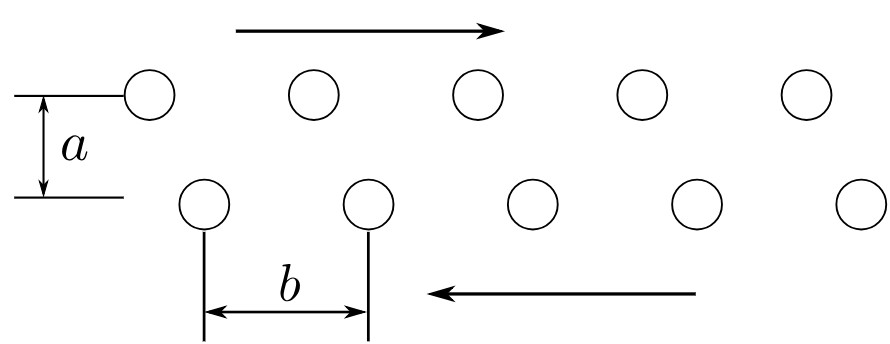
\includegraphics[width=0.7\textwidth]{fig/deformation_of_ideal_crystal.jpg}
                \caption{理想晶体变形示意图。}
                \label{理想晶体变形示意图}
            \end{figure}
            
            假定变形所受到的阻力为
            \begin{equation}
                \tau=\tau_m\sin{\left( \frac{2\pi x}{b} \right)}
            \end{equation}
            当发生的变形很小时,可以近似为
            \begin{equation}
                \tau=\tau_m{\left( \frac{2\pi x}{b} \right)},
            \end{equation}
            而且开始变形时,晶体处于弹性阶段,应当满足虎克定律,也就是
            \begin{equation}
                \tau=\mu\gamma=\mu\frac{x}{a},
            \end{equation}
            其中$\mu$为切变模量,$\gamma$为切应变,因此可以得到最大切应力为
            \begin{equation}
                \tau_m=\frac{\mu b}{2\pi a},
            \end{equation}
            由于本课程讨论的晶体绝大多数情况为简单立方晶系,可以认为$a=b$,所以最大切应变为
            \begin{equation}
                \tau_m=\frac{\mu}{2\pi}.
            \end{equation}

            然而理论切变强度$\frac{\mu}{2\pi}$与实际强度相比,实在太大。在使用更为合适的原子间作用力模型后,改变了正弦近似,
            最大切应变数值上降低为原来的$1/60$,但是这仍然比实际值高出了3到4个数量级。

            然而无论如何都提高应力模型的精确程度,最终结果的偏差仍然很大,因此是假设出现了问题。最终人们提出了位错模型,并且在
            实验中观察到了这一现象。
        
    \section{位错的结构}
        晶体中存在三种不同的位错类型,下面将分别描述。
            \subsection{刃型位错}
                考虑一个简单立方晶体,它在$(010)$面上沿$[100]$方向发生滑移,但是这个滑移是不均匀的。
                也就是从晶体的右侧向左传播。在某一时刻,滑移停止在晶体内部。于是在这个$(010)$面左右就可以划分出已滑移区域和未滑移区域,
                该面也就是两个区域的边界。晶体滑移的元过程是在一定的晶体学面上,沿一定的晶体学方向,晶体的上下两部分相对滑移一个或着多个
                点阵常数的距离。

                由此显然可见,已滑移的地区与未滑移的地区是一样的,上述滑移平面上下原子列是恢复对齐的,也就是说,这些地方恢复了理想晶体的长程
                有序性。所以除去\autoref{刃型位错形成示意图}中$\perp$的位置外,晶体的其他部分都是完整的。在这一区域内,晶体的完整周期性显然被
                破坏,所以这就是一个晶体缺陷,称为位错\index{位错}。
                \begin{figure}[ht]
                    \centering
                    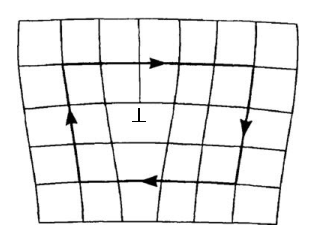
\includegraphics[width=0.45\textwidth]{fig/b_edge_dislocation.eps}
                    \caption{刃型位错形成示意图。}
                    \label{刃型位错形成示意图}
                \end{figure}

                关于位错最为简单的定义就是:位错是近完整晶体中的一个缺陷,是晶体中已滑移区和未滑移区的边界。
                
                这个边界更为严格的说,是分界区域的中心轴线,是平行于$[011]$方向的一条直线,其与滑移矢量$[100]$垂直,那么
                这个位错就称为刃型位错。

                上述中心轴线称为位错线\index{位错线},原理位错线的区域保持理想晶体的完整性;只有极为接近位错线的区域,也就是上述分界区域或
                过渡区域,晶体的点阵结构,或者原子的规则排列被破坏这一区域称为位错核心\index{位错!位错核心}。位错核心的半径与位错线的长度
                相比非常小,所以说,位错是晶体中的线性缺陷。

                对于刃型位错\index{位错!刃型位错},其与滑移矢量垂直,而\autoref{刃型位错形成示意图}中,$\perp$符号代表多余的一个半原子面,
                这个半原子面的边缘就是刃型位错的位错线,形状类似刀刃,因此称为刃位错\index{位错!刃位错}。
                因此刃型位错的形成也可以认为是一个半原子面中断与晶体内部,该边缘也就是一个刃型位错。

                在规定分割面的上下后,半原子面在割面上方的位错称为正刃型位错,反之则为负刃型位错,但是两者并没有本质上的区别。

                刃型位错有以下结构特点
                \begin{itemize}
                    \item[1] 位错周围有弹性畸变或非弹性畸变,上半部分晶体受压力,下部分受张力,中心为最大畸变,畸变局限在2或3个原子间距的管道内,总体为线缺陷;
                    \item[2] 位错线与滑移方向垂直;
                    \item[3] 上下晶体有一个相对位移$\vec{b}$,称为伯格斯矢量或简称柏式矢量\index{柏式矢量}。
                \end{itemize}
            \subsection{螺型位错}
                仍然假定滑移面为$\left( 010 \right)$面,位错线仍然是沿$[001]$方向的直线,但是滑移方向变为$[001]$方向,
                即为与位错线平行的方向,仍然将晶体分为已滑移区、未滑移区以及中间的过渡地带。同样,整个晶体是近完整的,只有在位错核心区,晶体的点阵
                结构才遭到破坏。
                
                也就是说,这也是一个二维缺陷,但是原子排列方式与刃型位错却不相同,不难得出,对与位错线垂直的原子面
                在位错不存在时,是一组彼此平行分立的平面,当此位错存在时,他们则变成一个连续的螺旋面。
                若绕此位错线以左手螺旋正向环行一周,即从一个面上升到相邻的另一个原子面,由于这个形质,这种位错称为螺型位错\index{位错!螺位错}。
                
                \begin{figure}[ht]
                    \centering
                    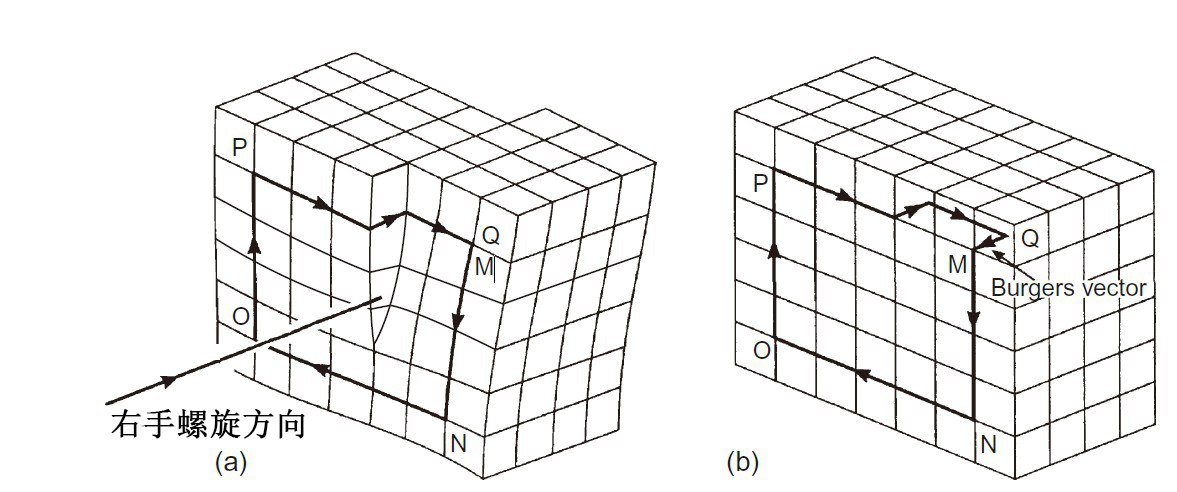
\includegraphics[width=0.7\textwidth]{fig/scheme_of_screw_dislocation.jpg}
                    \caption{右螺型位错示意图,(a)螺型位错的右手螺旋回路,(b)为相同回路在理想晶体中的绕行状况。}
                    \label{螺型位错示意图}
                \end{figure}

                在规定位错线正方向后,若绕位错线以右手螺旋方向绕行一周后,可以上升一个原子面的位错为右螺型位错,如\autoref{螺型位错示意图}
                若绕位错线以左手螺旋方向绕行一周后,可以上升一个原子面的位错为左螺型位错。
                左螺型位错和右螺型位错的滑移矢量方向也是相反的。

                在含有螺型位错的晶体中,原子面排布如\autoref{右螺型位错原子面排布}所示。晶体不再是刃型位错的附加半原子面,而是变成了螺旋式的曲面。
                \begin{figure}[ht]
                    \centering
                    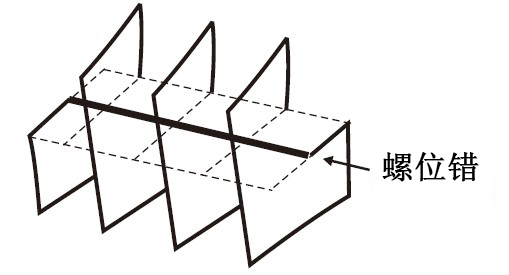
\includegraphics[width=0.5\textwidth]{fig/arrangement_of_atom_in_screw_dislocation.jpg}
                    \caption{右螺型位错原子面排布。}
                    \label{右螺型位错原子面排布}
                \end{figure}
            \subsection{混合型位错}
                然而一根直线位错可能既不与滑移矢量$\vec{b}$垂直,也不平行,而是成一个角度$\theta$,则这个位错既不是纯刃型位错也不是纯螺型位错,
                它可以看作是两个直线位错的叠加,分别为纯刃型和纯螺型的位错,两者的滑移矢量大小为
                \begin{align}
                    \vec{b}_1&=\vec{b}\sin\theta,\\
                    \vec{b}_2&=\vec{b}\cos\theta.
                \end{align}
                这个直线位错称为混合位错\index{位错!混合位错}。组成混合位错的两个分量为刃型分量和螺型分量。

                对上述情况加以推广,假设滑移矢量为$\vec{b}$,已滑移区域为\autoref{混合型位错的滑移示意}中的阴影部分,而位错线为图中红色线,从垂直与滑移面的方向看去,上下两个原子
                面之间的原子排布应该为\autoref{混合型位错的原子排列示意图}所示。
                \begin{figure}[ht]
                    \centering
                    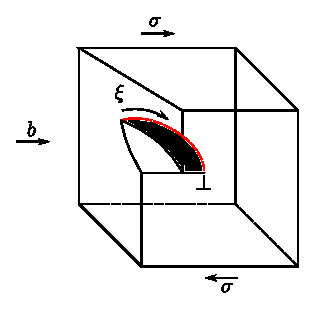
\includegraphics[width=0.5\textwidth]{fig/slip_of_mixed_dislocations.eps}
                    \caption{混合型位错的滑移示意。}
                    \label{混合型位错的滑移示意}
                \end{figure}
                
                \begin{figure}[ht]
                    \centering
                    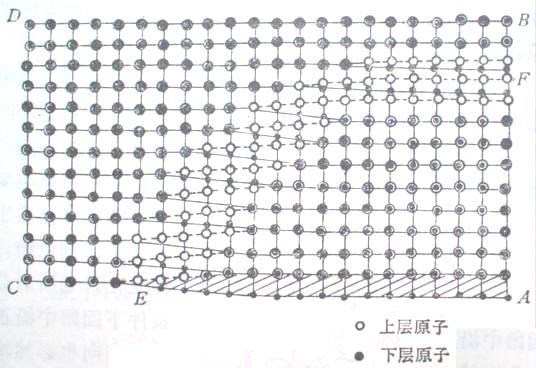
\includegraphics[width=0.5\textwidth]{fig/arrangement_of_atoms_of_mixed_dislocations.jpg}
                    \caption{混合型位错的原子排列示意图。}
                    \label{混合型位错的原子排列示意图}
                \end{figure}
                从\autoref{混合型位错的原子排列示意图}可以看出,这个位错有一段是纯螺型位错,另一端是纯刃型位错,由于位错线是连续的\footnote{这一点需要会证明。}
                从晶体的一个表面延伸到另一个表面,中间弯曲的一端既不是螺型位错也不是刃型位错,而是同时具有螺型和刃型位错的特征。
                这一小段也可以看作是许多方向近连续变化的小直线段所组成,每一小段都是混合型位错,各有一个螺型分量和刃型分量。
            \subsection{小结}
                依照以上定义,位错是晶体中滑移面上两个区域(即已滑移区域和未滑移区域)之间的分界,那么它就应该具有两个重要的性质:
                \begin{itemize}
                    \item[1] 因为晶体的滑移矢量是一个恒定矢量,等于一个或多个最小点阵平移矢量,所以对于一条位错线的各个部分,滑移矢量均相等;
                    \item[2] 无论位错线形状如何,总之位错线绝不可能终止于晶体的内部,位错线只能从晶体的一个表面延伸到另一个表面,或是在晶体中形成一个封闭的环。
                \end{itemize}
        \section{位错的普遍定义与伯格斯矢量}\label{section:位错的普遍定义与伯格斯矢量}
            \subsection{位错的普遍定义}
                在直观的基础上对位错的几何性质有一定的了解以后,我们这里可以对位错作出更为普遍的定义。

                假设晶体沿任意面$S$剖开,将$S$面的两边$S_1$以及$S_2$作一刚性的相对位移$\vec{b}$,$\vec{b}$可以是
                晶体中任意的电子平移矢量\footnote{$\vec{b}$不是点阵矢量的情形将在以后做出讨论。},经过这样的操作以后,
                如果$\vec{b}$与$S$面不平行,有些地方将产生原子位置重叠或者是空隙。去掉重叠的原子,空隙按照晶格排列填补,
                这样$S$面不会有任何改变,但是晶体中出现相对位移和未相对位移区域的分界线,也就是$S$面的周界。在分界线上原子错排的情况就是
                位错线\index{位错线},$\vec{b}$为伯格斯矢量或柏式矢量\index{柏式矢量},其为位错特征的标志,数值大小为$b$,
                称为位错的强度\index{位错!强度}。

                晶体中任意的位错都可以按照上面操作来形成, 但是汽油有一些需要注意的地方:
                \begin{itemize}
                    \item[1] 上述的想象操作不仅是用来说明位错的特征,也模拟了晶体产生位错的实际过程,关于位错生成的过程将以后讨论;
                    \item[2] 对于同一根位错线,可以有不同的$S$面,只要柏式矢量相图,形成的就是相同的位错,因此决定位错特征的是伯格斯矢量,而不是$S$面的具体位置,可以选以位错为边界的任意面作为上述操作的$S$面,比如沿$z$轴的刃型位错,选取$xoz$面和$yoz$面的结果是一致的;
                    \item[3] 实际上,从已经做过相对位移的区域到未作相对位移的区域间的过渡不可能是突变的,否则将产生无法填补的裂缝,因此$S$面两侧的刚性位移在边界是不再适用的,准确到说,位错不是一根线,而是有一定宽度$w$的区域,在这个区域内,$b$从中心的最大值下降到边界的零,只是由于宽度比长度小得多,所以可以近似为一根线。
                \end{itemize}
    
                \subsection{柏式矢量的定义}
                    $\vec{b}$矢量称为柏式矢量,它是位错线特征的标志,位错的强度为$b$,而方向的确定常使用伯格斯回路法和Frank惯例法。
                    \subsubsection{伯格斯回路法}
                        实现选取有位错的实际晶体,从好区中任意原子出发,微扰位错作一个闭合回路,回路每一步都连接相邻的同类原子,并且始终走在晶体的好区,这个回路称为伯格斯回路\index{伯格斯回路}。
                        然后在完整晶体中作一个对应的回路,即在相同方向走相同步数,结果发现这个回路无法闭合。终点到起点的矢量$\vec{b}$为柏式矢量\index{柏式矢量},回路
                        的方向与位错线方向成右手螺旋的方向为正方向。

                        假设晶体中三个基矢量$\vec{a}_0$,$\vec{b}_0$,$\vec{c}_0$,整个晶体的矢量都可以使用这三个矢量表示。
                        在理想晶体中,绕行晶体一周后必然有
                        \begin{equation}
                            \sum_{a}n_a\vec{a}_0+\sum_{c}n_b\vec{b}_0+\sum_{c}n_c\vec{c}_0=0\label{完整晶体的绕行结果},
                        \end{equation}
                        其中$n$为整数。

                        假如晶体不是完善的而是含有点缺陷,\autoref{完整晶体的绕行结果}仍然成立,但是基矢量在不同地方的长度有弹性范围内的差异,
                        这是因为点缺陷附近有弹性畸变,离开点缺陷稍远的地方,弹性畸变相应减少。

                        加入这个封闭回路本身经过的地方都是良好的,但是回路包围的区域中含有一个位错$\vec{b}$,回路的方向与位错的方向构成右手螺旋关系,对这个回路,\autoref{完整晶体的绕行结果}变为
                        \begin{equation}
                            \sum_{a}n_a\vec{a}_0+\sum_{c}n_b\vec{b}_0+\sum_{c}n_c\vec{c}_0=-\vec{b},                            
                        \end{equation}

                    \subsubsection{Frank惯例法}
                        Frank惯例法\index{Frank惯例法}需要线确定位错线的正向,割面及割面法线的正向,按照右手螺旋定则,四个手指顺位错线垂直防御割面上,大拇指指向正半晶体也就是法线方向,规定$\vec{b}$为
                        负半晶体相对与正半晶体的移动方向。

                        在确定$\vec{b}$后,如果位错线与$\vec{b}$平行,则为螺旋位错,方向相同为正,反向为负;如果$\vec{b}$与位错线垂直,
                        则为刃型位错,对于刃型位错的方向,需要使用半原子面右手法,如\autoref{刃型位错的半原子面右手法则}所示。
                        \begin{figure}[ht]
                            \centering
                            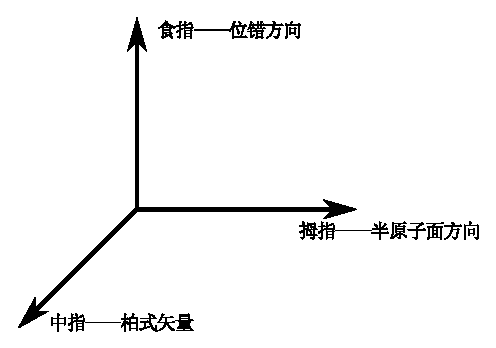
\includegraphics[scale=1]{fig/right_hand_rule_of_edge_dislocation.eps}
                            \caption{刃型位错的半原子面右手法则。}
                            \label{刃型位错的半原子面右手法则}
                        \end{figure}
                \subsection{柏式矢量守恒定律}
                        利用柏式回路的概念即可论证伯格斯矢量的守恒定律:
                        \begin{enumerate}
                            \item[1] 一个位错线不可能中止于晶体内部,它必然构成闭合1的圈或终止于晶体表面,沿一根不分岔的位错线的伯格斯矢量是守恒的,具有相图的大小和方向。
                            \item[2] 如果数根位错线相较于一点,此点称为位错的节点\index{节点},朝向节点的各位错线柏式矢量的总和等于流出各节点位错线伯格斯矢量矢量的总和,如果所有的位错线方向都是从节点出发,则上述关系可以写作各分支柏式矢量的总和为零,即$\sum b=0$;
                            \item[3] 柏式回路有如下特点:
                            \begin{enumerate}
                                \item[1)] 一根位错线只有一个柏式矢量;
                                \item[2)] 位错线不能在晶体内部中断,因而它们只能或者终止在晶体表面,或者形成封闭环,或者与其它位错相联;
                                \item[3)] 当位错与其它位错相联时,指向结点的位错柏氏矢量和与离开节点位错的柏氏矢量和相等,若均指向一个节点,有$\sum b=0$。
                            \end{enumerate} 
                        \end{enumerate}
        
        \section{位错应力场}
            根据\autoref{section:位错的普遍定义与伯格斯矢量},位错是一个线缺陷,其最大畸变分布在以位错线为轴心的管道区域内,管道的直径为2到3个原子间距。
            同时位错的畸变与距离位错线的距离成反比,距离越远的区域,畸变也越小。
            但是由于位错造成的畸变遍布整个晶体,所以伴随这些畸变也造成了晶体各原子之间的位置发生变化,偏离了
            原来的平衡位置,相互之间产生了内应力的作用,应力和应变的乘积即是造成系统能量上升的原因,因此需要定量地分析位错在晶体中所引起的畸变
            和能量。

            为了方便研究,一般把晶体分成两个区域
            \begin{itemize}
                \item[1] 位错中心,由于这个区域畸变严重,必须要考虑晶体结构和原子间相互作用,才能分析应力场和相应的能量;
                \item[2] 远离位错中心的区域,这一部分畸变相对较小,因此可以使用线弹性理论处理。
            \end{itemize}
            
            如\autoref{螺型位错的连续介质模型}所示,沿$z$方向位错线取一个圆柱体,由于中心位置畸变能过大,将其中心挖去,挖掉的区域半径为$r_0$。
            圆柱体沿$z$方向错开一个原子间距$b$,也就是晶体中出现了一个螺位错。假设所研究的点距离中心为$r$,则在绕行一周后,弹性畸变为$b$,平均单位周长变形为
            \begin{equation}
                \varepsilon=\frac{b}{2\pi r}.
            \end{equation}

            \begin{figure}[ht]
                \centering
                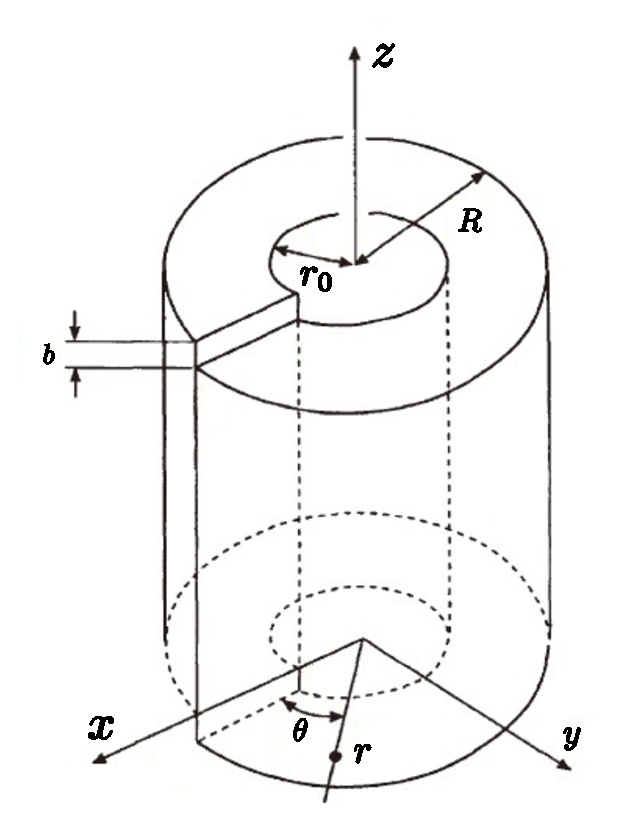
\includegraphics[scale=0.5]{fig/continuous_model_of_screw_dislocation.eps}
                \caption{螺型位错的连续介质模型。}
                \label{螺型位错的连续介质模型}
            \end{figure}

            在柱坐标系中,平均单位周长变形为
            \begin{equation}
                \gamma_{z\theta}=\frac{b}{2\pi r},
            \end{equation}
            由于是弹性变形,代入到胡克定律中,有
            \begin{equation}
                \tau_{z\theta}=\mu\gamma=\frac{\mu b}{2\pi r}, r>r_0.
            \end{equation}
            其中$\mu$为切变模量。

            在直角坐标系中,可以得出
            \begin{align}
                \tau_{xz}&=-\frac{\mu b}{2\pi}\frac{y}{x^2+y^2},\\
                \tau_{yz}&=\frac{\mu b}{2\pi}\frac{x}{x^2+y^2},
            \end{align}
            由此可以看出,
            \begin{itemize}
                \item[1] 在晶体中,只要有位错就有应力场,而不管此晶体是否有外加应力,外加应力与位错产生的应力场无关;
                \item[2] 不同$r$都有应力场,也就是说,位错应力是一个长程应力场,遍布于整个晶体的应力场;
                \item[3] 伴随$r$增大,$\tau$减小,因此距离位错中心越远的地方,应力也就越小;
                \item[4] 根据公式的结果,$r$趋于0,$\tau$为无限大,因此上述公式不再适用于这种情况,这与挖掉位错核心这一方法相符。
            \end{itemize}
            关于位错的应力场的分布则主要是弹性力学的内容,这里不再关注。

            \subsection{刃型位错的应力场}
                假设晶体没有边界,体积无限大,刃位错的位错线沿$z$方向,符号为正,如\autoref{刃型位错的连续介质模型}所示,则
                \begin{figure}[ht]
                    \centering
                    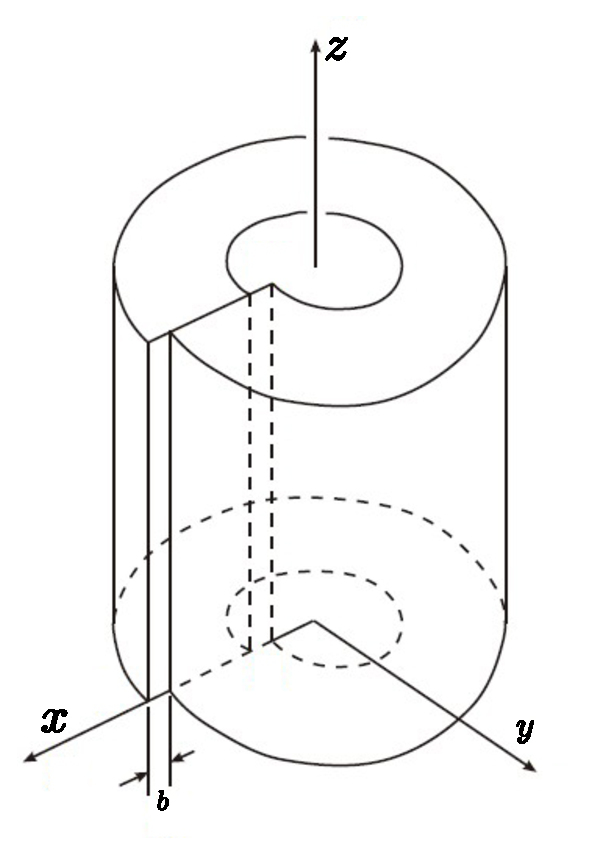
\includegraphics[scale=0.5]{fig/model_of_edge_dislocation.eps}
                    \caption{刃型位错的连续介质模型。}
                    \label{刃型位错的连续介质模型}
                \end{figure}
                应力场的主应力及分量为:
                \begin{align} 
                    \sigma_{x x} &=-\frac{\mu b}{2 \pi(1-v)} \frac{y\left(3 x^{2}+y^{2}\right)}{\left(x^{2}+y^{2}\right)^{2}}\label{刃位错的x主应力}, \\ 
                    \sigma_{y y} &=\frac{\mu b}{2 \pi(1-v)} \frac{y\left(x^{2}+y^{2}\right)}{\left(x^{2}+y^{2}\right)^{2}}\label{刃位错的y主应力}, \\
                    \tau_{x y} &=\frac{\mu b}{2 \pi(1-v)} \frac{x\left(x^{2}-y^{2}\right)}{\left(x^{2}+y^{2}\right)^{2}}\label{刃位错的切应力}, \\
                    \sigma_{z z} &=v\left(\sigma_{x x}+\sigma_{y y}\right)\label{刃位错的z主应力}, \\
                    \tau_{x z} &=\tau_{y z}=0 .
                \end{align}
                其中$v$为泊松比,改用柱坐标系后上述关系变为
                \begin{align}
                    \sigma_{r r}&=\sigma_{\theta \theta}=-\frac{\mu b}{2 \pi(1-v)} \frac{\sin \theta}{r}, \\ 
                    \sigma_{r \theta}&=\frac{\mu b}{2 \pi(1-v)} \frac{\cos \theta}{r}, \\ 
                    \sigma_{z z}&=v\left(\sigma_{r r}+\sigma_{\theta \theta}\right).
                \end{align}
                从刃型位错应力场的表达式可以发现,刃型位错有以下特点
                \begin{enumerate}
                    \item[1] 应力场与$z$方向无关,是平面型的;
                    \item[2] 正应力场关于$yoz$面和$y$轴对称,而且$|\sigma_{xx}|>|\sigma_{yy}|$,
                    \begin{enumerate}
                        \item[a] 当$y>0$也就是上半晶体,$\sigma_{xx}<0$,受压应力,
                        \item[b] 当$y<0$也就是下半晶体,$\sigma_{xx}>0$,受张应力;
                    \end{enumerate} 
                    \item[3] 应力大小与$b$大小有关,而且当$r$增大,应力下降,这与简化分析得到的结果一致;
                    \item[4] $y=0$时,$xoz$面也就是位错的滑移面上有
                            \begin{align}
                                \sigma_{xx}&=\sigma_{yy}=0,\\
                                \tau_{xy}&=\tau_{yx}.
                            \end{align} 
                            也就是切应力在滑移面上有最大值。
                \end{enumerate}
            \subsection{螺型位错的应力场}
                在直角坐标系下,\autoref{螺型位错的连续介质模型}的应力场表达形式为
                \begin{align} 
                    \tau_{x z} &=-\frac{\mu b}{2 \pi} \frac{y}{x^{2}+y^{2}}, \\
                    \tau_{y z} &=\frac{\mu b}{2 \pi} \frac{x}{x^{2}+y^{2}}. 
                \end{align}
                在柱坐标系下,有
                \begin{equation}
                    \tau_{\theta z}=\tau_{z\theta}=\frac{\mu b}{2\pi r},
                \end{equation}
                而其他的应力分量均为0。而螺型位错的应力场的特点为
                \begin{itemize}
                    \item[1]  螺型位错的应力场只有切应力分量,没有正应力分量,所有的正应力分量均等于0。
                    \item[2] 应力大小和$b$有关,并且随着$r$越大、应力越小;
                    \item[3] 应力是轴对称的,与$θ$无关。
                \end{itemize}
            \subsection{混合位错的应力场}
                混合型位错可以采用将柏氏矢量分解的办法进行求解,我们可以发现,位错线平
                行的螺型位错由于没有正应力分量,因此其正应力分量只要采用刃型位错的正应力分
                量即可。
                
                同时刃型位错的切应力分量只有$\tau_{xy}$分量,而螺型位错的切应力分量为$\tau_{xz}$和$\tau_{yz}$,
                因此没有相互重叠的应力分量,可以进行叠加。因此可以总结为如下的特点:
                \begin{itemize}
                    \item[1] 螺型和刃型没有重叠分量;
                    \item[2] 应力场互不影响;
                    \item[3] 因此混合型可以分解为螺型与刃型分量分别计算并叠加。
                \end{itemize}
        \section{位错的应变能}
            前一章已经求出位错的应力场和畸变分布,可以得到,晶体中弹性能量密度为
            \begin{equation}
                \frac{1}{2}\sigma_{ij}\varepsilon-{ij},
            \end{equation}
            由于位错的应力场分为两部分来求解,因此对于位错能量也分为两部分,一部分为位错的核心能量,一部分为周围应力场的能量,也就是应变能,
            利用弹性能量密度,可以得到单位立方体总的应变能
            \begin{equation}
                w=\frac{1}{2}\left(\sigma_{x} \varepsilon_{x}+\sigma_{y} \varepsilon_{y}+\sigma_{z} \varepsilon_{z}+\tau_{x y} \gamma_{x y}+\tau_{y z} \gamma_{y z}+\tau_{z x} \gamma_{z x}\right),
            \end{equation}
            整个弹性题的应变能为
            \begin{equation}
                W=\frac{1}{2}\iiint\sigma\varepsilon\dif v,
            \end{equation}
            但是这一过程非常复杂,求解难度很大。然而采用做功法,利用位错的形成过程,计算这个过程中所做的功,也就是系统能量的增加。

            \subsection{刃型位错的应变能}
                刃型位错形成时可以看作上下半晶体相互推移$\alpha b$,其中$\alpha$在0和1之间,在$\theta=0$处的切应力为
                \begin{equation}
                    \sigma_{\theta r}=\sigma_{r \theta}=\frac{\mu\alpha b}{2\pi(1-v)}\cdot\frac{1}{r},
                \end{equation}
                形成单位长度的位错,做功为
                \begin{equation}
                    \begin{aligned}
                        \dif w&=\frac{\mu\alpha b}{2\pi(1-v)}\cdot\frac{1}{r}\dif r\cdot\dif(\alpha b),\\
                            &=\frac{\alpha\mu b^2}{2\pi(1-v)r}\dif r\dif \alpha,
                    \end{aligned}
                \end{equation}
                对体积元积分,可以得到整个晶体的位错做功
                \begin{equation}
                    \begin{aligned}
                        w_{\text{刃}}&=\int_{r_0}^{r_1}\int_{0}^{1}\frac{\alpha\mu b^2}{2\pi(1-v)r}\dif r\dif \alpha\\
                        &=\frac{1}{2}\alpha^2\lvert_{0}^{1}\cdot\int_{r_0}^{r_1}\frac{\mu b^2}{2\pi(1-v)r}\dif r\\
                        &=\frac{1}{2}\cdot\frac{\mu b^2}{2\pi(1-v)}\ln\left( \frac{r_1}{r_0} \right).
                    \end{aligned}
                \end{equation}
                由于圆柱体内外表面均为自由面条件,因此应该进行修正,修正公式为
                \begin{equation}
                    w_{\text{刃}}\simeq\frac{\mu b^2}{2\pi(1-v)}\left[ \ln\left( \frac{r_1}{r_0} \right) -1\right],
                \end{equation}
                当远离位错核心时,即$r_1\gg r_0$时,这种修正就不重要了。
            \subsection{螺型位错的应变能}
                对于螺型位错的处理与刃型位错的处理接近,晶体之间相互移动$\alpha b$,晶体之间切应力为
                \begin{equation}
                    \sigma_{\theta z}=\frac{\mu\alpha b}{2\pi r},
                \end{equation}
                切应力做功为
                \begin{equation}
                    \begin{aligned}
                        w_{\text{螺}}&=\int_{r_0}^{r_1}\int_{0}^{1}\sigma_{\theta z}b\dif r\dif \alpha\\
                        &=\int_{r_0}^{r_1}\int_{0}^{1}\frac{\mu b^2}{2\pi r}\dif r\alpha\dif \alpha\\
                        &=\frac{\mu b^2}{2\pi r}\ln\left( \frac{r_1}{r_0} \right).
                    \end{aligned}
                \end{equation}
                修正后为
                \begin{equation}
                    w_{\text{螺}} =\frac{\mu b^2}{2\pi r}\left[ \ln\left( \frac{r_1}{r_0} \right)-1 \right].                    
                \end{equation}
            \subsection{混合型位错的应变能}
                由于混合型位错的应力场可以将混合型位错分解为螺型分量和刃型分量再求出各
                自的应力场分量后进行叠加,从而应变能也可以先分解,再进行叠加即可。

                假设柏式矢量$\vec{b}$与位错线夹角等于$\psi$,则刃型位错和螺型位错的分量为
                \begin{align}
                    \text{刃型位错:}&b_\perp=\vec{b}\sin\psi,\\
                    \text{螺型位错:}&b_\parallel=\vec{b}\cos\psi.\\                
                \end{align}
                由于同向刃型位错与螺型位错无相互作用,两者可以叠加
                \begin{equation}
                    w_{\text{混}}=\frac{\mu b^{2} \sin ^{2} \psi}{4 \pi(1-v)} \ln \left(\frac{r_{1}}{r_{0}}\right)+\frac{\mu b^{2} \cos ^{2} \psi}{4 \pi} \ln \left(\frac{r_{1}}{r_{0}}\right),
                \end{equation}
                或者写为:
                \begin{align}
                    w_{\text{混}}=\frac{\mu b^{2}}{4 \pi K} \ln \left(\frac{r_{1}}{r_{0}}\right),\\
                    \frac{1}{K}=\cos^2\psi+\frac{\sin^2\psi}{1-v}.
                \end{align}
                从应变能的表达式可以看出:
                \begin{itemize}
                    \item[1] 应变能和$b^2$成正比,刃型比螺型差一个因子,由于一般金属材料泊松比在0.3左右,也就是说,相同位错强度的刃型位错比螺型位错的应变能大50\%左右;
                    \item[2] 接近位错核心时,公式不再适用,通常情况下,位错核心能是应变能的十分之一;
                    \item[3] 对于一般金属,位错应力场范围受到亚晶界的限制,所以$r_1\simeq\SI{1e-4}{\cm}$,而$r_0\simeq\SI{1e-8}{\cm}$,因此在原理位错核心区有
                    \begin{equation}
                        w_{\text{混}}\simeq\mu b^2=\alpha\mu b^2,
                    \end{equation} 
                    其中$\alpha$在\numrange{0.5}{1}之间,因为位错的应变能相当大,在位错的自由能的表达式
                    中,应变能是主要的项,所以位错不是热平衡自由能最低的产物,这一点和空位不
                    同。
                \end{itemize}
        \section{位错的线张力}
            已知位错的能量与它的长度成正比,若要增加位错的长度,必须做功,因此,围殴错总是有收缩其长度的趋势,
            这表明在能量的意义上将,位错线表现有线张力。可以定义位错线张力等于位错线伸长一个单位长度所做的功,
            用$T$表示。一个直位错的张力等于
            \begin{equation}
                \begin{aligned}
                    T&=\frac{\partial W}{\partial l}\\
                    &=\frac{\mu b^{2} \sin ^{2} \psi}{4 \pi(1-v)} \ln \left(\frac{r_{1}}{r_{0}}\right)\left(1-v \cos ^{2} \psi\right)\\
                    &\simeq \frac{1}{2}\mu b^2.
                \end{aligned}
            \end{equation}
            但是,位错的张力多少和位错的形状有关,上式所指的是直的位错。对于一般波
            浪形的位错,其张力基本上也可以用式,证明从略。故在以后的应用中均用此公式表
            示位错的线张力。
        \section{位错核心}
            在讨论应力场和应变能的时候,都提到由于位错核心\index{位错核心}区域的畸变太大,不能用线弹性理论来求解,必须引入点阵的周期性,并结合连续
            介质的结果处理一系列问题:位错核中心的宽度,位错在点阵中运动的阻力和位错中心能量的问题。

            但是点阵模型不是彻底的,仍然要采纳某些观点和结果,所以只使用一个半点阵模型。

            这一节的点阵模型最早由Peiels提出,后来Nabarro对这一模型进行了修正,因此称为
            Peiels-Nabarro模型,简称派-纳模型\index{位错核心!派-纳模型}。
            \subsection{点阵模型}
                以简单立方晶体的刃型位错为例,位错可以视为由两个完成的半晶体拼接而成。
                \begin{figure}[ht]
                    \centering
                    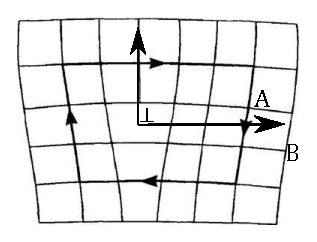
\includegraphics[width=0.5\textwidth]{fig/coordinate_in_edge_dislocation.eps}
                    \caption{刃型位错模型。}
                    \label{刃型位错模型}
                \end{figure}

                设原子间距为$\Phi$,在拼合之前,横轴方向的原子间距为
                \begin{equation}
                    \begin{aligned}
                        \Phi&=\frac{1}{2}b,x>0,\\
                        \Phi&=-\frac{1}{2}b,x<0.
                    \end{aligned}
                \end{equation}
                在拼合后,上下两层分别受到压力和张力,使得原子尽量对齐,在这一过程中,假设上半晶体中位错核心层的
                原子发生了位移$u(x)$,则有
                \begin{equation}
                    \begin{aligned}
                        x>0,u(x)<0,\\
                        x>0,u(x)>0.
                    \end{aligned}
                \end{equation}
                而原子间距则变为
                \begin{align}
                    \Phi(x)=2u(x)+\frac{b}{2},x>0\label{位错正向的原子的位移},\\
                    \Phi(x)=2u(x)-\frac{b}{2},x<0.
                \end{align}
                距离位错核心无穷远时,位错的影响忽略不计,也就是$\Phi(\pm\infty)=0$,所以有
                \begin{equation}
                    u(\infty)=-u(-\infty)=-\frac{b}{4}.
                \end{equation}
                \begin{figure}[ht]
    \centering
    \begin{tikzpicture}
        \begin{axis}[
            xlabel={$x$},
            ylabel={$u(x)$},
            xtick=\empty,
            ytick=\empty,
            axis y line =center,
            axis x line =center,
        ]
            \addplot[blue,thin,domain=0:5,samples=100] {exp(-x)-1};
            \addplot[blue,thin,domain=-5:0,samples=100] {-exp(x)+1};
            \addplot [black,thin,dashed,domain=-5:5] {1.08}
                node [pos=0.75,anchor=north] {$\frac{b}{4}$};
            \addplot [black,thin,dashed,domain=-5:5] {-1.08}
                node [pos=0.25,anchor=south] {$-\frac{b}{4}$};
        \end{axis}
    \end{tikzpicture}
    \caption{原子平衡位置的偏离与位错核心距离的关系。}
    \label{原子平衡位置的偏离与位错核心距离的关系}
\end{figure}

                为求出相应的位移,以及各个原子之间的畸变,Peierls假定上下两层之间的作用力为周期性,
                位错管道外为连续介质,这样,两层原子之间的吸引产生了切应力$\sigma_{yx}$,
                \begin{equation}
                    \sigma_{yx}=\frac{\mu}{2\pi}\left( \frac{b}{a} \right)\sin\left( \frac{2\pi\Phi}{b} \right),x>0,
                \end{equation}
                代入\autoref{位错正向的原子的位移},可得
                \begin{equation}
                    \sigma_{yx}=-\frac{\mu}{2\pi}\left( \frac{b}{a} \right)\sin\left( \frac{4\pi u(x)}{b} \right),x>0,                    
                \end{equation}
                当$\Phi$很小时,没有发生塑性形变,因此可以使用虎克定律
                \begin{equation}
                    \sigma_{yx}=\frac{\mu}{2\pi}\left( \frac{b}{a} \right)\sin\left( \frac{2\pi\Phi}{b} \right)=\mu\left( \frac{\Phi}{a} \right)\label{刃位错核心引起的切应力公式1}.
                \end{equation}

                同时为了求出上半部材料的切应力,EShelby提出柏式矢量为$\vec{b}$的位错可以
                看作是无穷小位错分布在滑移面上,柏式矢量之和等于$\vec{b}$,且分布不均匀。
                设分布在$x^{\prime}\to x^{\prime}+\dif x^{\prime}$之间的柏式矢量为$f(x^{\prime})$
                因此总的柏式矢量为
                \begin{equation}
                    \int_{-\infty}^{^\infty}f(x^{\prime})\dif x^{\prime}=\vec{b},
                \end{equation}
                分布在$x^{\prime}\to x^{\prime}+\dif x^{\prime}$之间的切应力为$\frac{\mu f(x^\prime)}{2\pi(1-v)}\cdot\frac{(x-x^{\prime})^3}{(x-x^\prime)^4}\dif x^{\prime}=\frac{\mu f(x^\prime)}{2\pi(1-v)}\frac{\dif x^{\prime}}{x-x^{\prime}}$
                在两层原子之间的切应力为
                \begin{equation}
                    \sigma_{y x}=\frac{\mu}{2 \pi(1-v)} \int_{-\infty}^{\infty} \frac{f\left(x^{\prime}\right) d x^{\prime}}{x-x^{\prime}}, x^{\prime}>0\label{利用不均匀位错导出的核心切应力1},
                \end{equation}
                当$x=x^\prime$时,有
                \begin{equation}
                    \dif u(x^\prime)=f(x^\prime)\dif x^\prime,
                \end{equation}
                \autoref{利用不均匀位错导出的核心切应力1}可以写作
                \begin{equation}
                    \sigma_{y x}=-\frac{\mu}{\pi(1-v)} \int_{-\infty}^{\infty} \frac{\frac{d u\left(x^{\prime}\right)}{d x^{\prime}} d x^{\prime}}{x-x^{\prime}}, x>0\label{刃位错核心引起的切应力公式2},
                \end{equation}
                
                联立\autoref{刃位错核心引起的切应力公式1}和\autoref{刃位错核心引起的切应力公式2},解得
                \begin{equation}
                    u(x)=-\frac{b}{2\pi}\arctan\left( \frac{x}{\xi} \right),\xi=\frac{a}{2(1-v)},
                \end{equation}
                当$x=0$,$u(x)=0$,而$\Phi=\frac{b}{2}$,在无穷远处,$u(x)=\frac{b}{4}$,此时$\Phi=0$,
                这与之前的结果一致。位错管道附近的错排值分布如\autoref{错排值沿滑移面的分布}所示。

                \begin{figure}[ht]
    \centering
    \begin{tikzpicture}
        \begin{axis}[
            xlabel={$x$},
            ylabel={$\left\vert\Phi\right\vert$},
            xtick=\empty,
            ytick=\empty,
            axis y line =center,
            axis x line =bottom,
            ymax=1.5,
        ]
            \addplot[blue,thin,domain=0:5,samples=100] {1-2*rad(atan(1.4*x))/3.1415}
                node[pos=0,black,anchor=east] {$\frac{b}{2}$};
            \addplot[blue,thin,domain=-5:0,samples=100] {1-2*rad(atan(-1.4*x))/3.1415};
            \addplot[dashed,black,domain=-0.75:0.75] {0.5}
                node[pos=0.35, anchor=north] {$\omega$};
        \end{axis}
    \end{tikzpicture}
    \caption{错排值沿滑移面的分布。}
    \label{错排值沿滑移面的分布}
\end{figure}
                
                从图中把畸变的半高宽定义为位错的宽度,因此位错的宽度为
                \begin{equation}
                    \omega=2\xi=\frac{a}{1-v},
                \end{equation}
                对于泊松比为0.3的材料,位错的宽度约为$1.5a$。
            \subsection{位错引起的晶体错排能}
                前面已经提到,用连续介质中位错的模型可以求出弹性畸变区的能量,但不能求
                出位错中心的能量。现在我们可以根据上述点阵模型对这部分能量做一个估计。位错
                总的应变能包括两部分,即$\omega_0$就是以前求过的弹性区的能量,$\omega_{AB}$
                是由于位错中心附近滑移面上下两层原子没能对齐的能量——错排能。

                由于错排实际只在位错附近,所以这部分能量属于位错中心区的能量。
                先求解弹性区的应变能$W_0$,根据点阵模型得到的应力表达式,代入后可以求得
                \begin{equation}
                    \begin{aligned}
                        W_{0}&=\frac{1}{2} \int_{\xi}^{r_{1}} \sigma_{y_{x}} b \dif x\\
                        &=-\frac{\mu b^{2}}{4 \pi a} \int_{\xi}^{r_{1}} \sin \frac{4 \pi u(x)}{b} \dif x\\
                        &=\frac{\mu b^{2}}{4 \pi a} \int_{\xi}^{r_{1}} \sin \left[2 \arctan\left(\frac{x}{\xi}\right)\right] \dif x
                    \end{aligned}
                \end{equation}
                由于位错是长程应力场,$r_1\gg\xi$,因此有
                \begin{equation}
                    W_0\simeq\frac{\mu b^2}{4\pi(1-v)}\ln\frac{r_1}{\xi}.
                \end{equation}
                然后求解错排能,在计算应变能时,假定位错宽度以外滑移面两侧的晶体发生
                刚性滑移,然而这在位错核心区不再适用,在上节计算错排能的时候,为了强调点阵模型.所以用代数的加
                法,这是为了要显示出位错偏离出对称位置以后能量的变化。做为近似,假如如不需
                要求点阵阻力,我们仍然可用积分代替相加两层的对应原子的错排能已知等于
                \begin{equation}
                    \frac{\mu b^{3}}{4 \pi^{2} a}\left(1+\cos \frac{4 \pi u(x)}{b}\right)=\frac{\mu b^{3}}{2 \pi^{2} a} \cos ^{2}\left(\frac{2 \pi u(x)}{b}\right)=\frac{\mu b^{3}}{2 \pi^{2} a} \cos ^{2}\left(\arctan \frac{x}{\xi}\right),
                \end{equation}
                错排能的表达式为
                \begin{equation}
                    W_{AB}\simeq\frac{\mu b^2}{2\pi(1-v)},
                \end{equation}
                这一数值与应变能相比,差了一个系数$\ln\left( \frac{r}{\xi} \right)$,如果$r=\SI{1e-4}{\cm}$,
                $\xi$为\SI{1e-8}{\cm},则可以计算处错排能大约为应变能的0.1。
            \subsection{点阵阻力}\label{subsection:点阵阻力}
                平衡的条件下,位错处于平衡位置,如果位错中心发生了$\alpha b$的滑移,系统的能量也会发生变化,
                这一变化的梯度造就了位错移动的阻力。这样,计算的关键在于求出位于位错偏离出对称位置时,由于滑
                移面上下两层原子没有对齐而引起的能量。假设\autoref{刃型位错模型}中AB两层原子对齐时作用能为零。
                考虑A层任意一行与纸面垂直的原子,这一行原子与位错平行,并且为单位长度,它所受的力$F$若按照
                连续介质的观点是分布在面积$b$上面的,
                这一行原子所受的力为
                \begin{equation}
                    F=\sigma_{xy}b\label{位错核心受到的力与柏式矢量关系},
                \end{equation}
                因此可以说这一行原子和B层对应原子因为没有对齐而具有能量,也就是错排能,其等于
                \begin{equation}
                    \frac{1}{2}\int_{0}^{\Phi}\sigma_{yx}b\dif \Phi,
                \end{equation}
                其中的系数$1/2$是因为原子之间的势能分配在A 和B 两部分的值将取自\footnote{这里有缺漏,希望有人补完。}
                。因此在A层与$z$轴平行的单位长度的一行原子具有的错排能为
                \begin{equation}
                    \begin{aligned}
                        V_{u(x)}&=-\frac{1}{2}\left(\frac{\mu b^{2}}{2 \pi a}\right) \int \sin \frac{4 \pi u(x)}{b} d(2 u) \\ 
                            &=-\frac{\mu b^{3}}{8 \pi^{2} a} \int \sin \frac{4 \pi u}{b} d\left(\frac{4 \pi u}{b}\right) \\ 
                            &=\frac{\mu b^{3}}{8 \pi^{2} a}\left(\cos \frac{4 \pi u}{b}\right)+C.
                    \end{aligned}
                \end{equation}
                $C$为积分常数,已知当$u=\pm\frac{b}{4}$时,错排能为零,可以求出$C$:
                \begin{equation}
                    C=-\frac{\mu b^{3}}{8 \pi^{2} a} \cos \left(\frac{4 \pi}{b} \cdot \frac{b}{4}\right)=\frac{\mu b^{3}}{8 \pi^{2} a},
                \end{equation}
                回代得到
                \begin{equation}
                    V_{u(x)}=\frac{\mu b^{3}}{8 \pi^{2} a}\left[1+\cos \frac{4 \pi u(x)}{b}\right].
                \end{equation}
                若位错正好位于对称位置,则A和B两层全部原则为位置可以写作
                \begin{equation}
                    x=\frac{1}{2}nb,n=0,\pm1,\pm2\cdots
                \end{equation}
                当位错中心发生$\alpha b$的位移后,原子位置近似可以表示为
                \begin{equation}
                    x=\left( \alpha+\frac{1}{2}n \right)b,
                \end{equation}
                这样错排能变为
                \begin{equation}
                    \begin{aligned}
                        V&=\frac{\mu b^{3}}{8 \pi^{2} a} \sum_{-\infty}^{+\infty}\left[1+\cos \frac{4 \pi}{b}\left\{-\frac{b}{2 \pi} \arctan \frac{\left(a+\frac{1}{2} n\right)}{\xi} b\right\}\right] \\
                        &=\frac{\mu b^{3}}{8 \pi^{2} a} \sum_{-\infty}^{+\infty}\left[1+\cos 2\left\{\arctan \frac{\left(a+\frac{1}{2} n\right)}{\zeta} b\right\}\right].
                    \end{aligned}
                \end{equation}
                单个原子的势能可以写作
                \begin{equation}
                    V_{\alpha}=\frac{\mu b^{2} \xi}{\pi a} \sum_{s=1}^{\infty} e^{-4 x \xi_{s} / b} \cos 4 \pi a s,
                \end{equation}
                将$\xi=\frac{a}{2(1-v)}$代入得到
                \begin{equation}
                    V_{a}=\frac{\mu b^{2}}{2 \pi(1-v)} e^{-4 \pi \xi / b} \cos 4 \pi \alpha,
                \end{equation}
                位错运动受到的力为
                \begin{equation}
                    F=\frac{-\partial V_\alpha}{\partial(\alpha b)}=\frac{-1}{b}\frac{\partial V_a}{\partial\alpha}=\frac{2\mu b}{1-v}e^{-\frac{4\pi\xi}{b}}\sin{4\pi\alpha},
                \end{equation}
                其最大值为$F_{\mathrm{max}}=\frac{2 \mu b}{1-\nu} e^{-4 \pi \xi / b}$。
                根据\autoref{位错核心受到的力与柏式矢量关系},刃位错运动受到的切应力为
                \begin{equation}
                    \sigma_{e}=\frac{2 \mu}{1-v} e^{\frac{-i \pi \xi} { b}}=\frac{2 \mu}{1-v} e^{ -\frac{2 \pi a}{b(1-v)}},
                \end{equation}
                称为点阵阻力\index{点阵阻力},也称作派-纳力。
            \subsection{小结}
                \begin{itemize}
                    \item 位错的核心能约为$\frac{1}{10}\mu b^2$,也就是应变能的$1/10$;
                    \item 位错的宽度认为是$\omega=1.5a$,$a$为晶格常数;
                    \item 点阵阻力$\tau$取决于点阵阻力$a$和柏式矢量$b$,当点阵常数增大时,阻力减小。
                \end{itemize}
        \section{位错的受力与运动}
            \subsection{位错的运动方式}
                晶体在受到适当的应力时,位错可以发生运动,其实在构造位错的示意中就可以
                发现,如果应力继续施加,实际产生的效果就是位错的滑移。位错的运动方式分为
                滑移和攀移。

                滑移指位错滑移在滑移面上的运动,滑移面是位错线和柏式矢量确定的平面,法线方向为$\vec{l}\times \vec{b}$。
                而攀移是指位错垂直于滑移面上的运动。对于这两种运动,下面将分为刃型位错和螺型位错讨论。

                对于刃型位错,滑移过程如\autoref{刃型位错滑移时周围原子的动作}所示,设晶体中已有一个刃型位错,在外加
                切应力作用下,这个位错发生运动,可使晶体上下发生相对移动的区域逐渐扩大。当位错移出晶体的时候就是获赠个晶体
                上下两部分已经完成了相对移动一个原子间距。表示随着刃型位错在晶体中扫过的各个阶段所造成的变形。是位错在晶体
                尚未移出晶外,位错扫过整个滑移面时,就会造成永久切变。
                \begin{figure}[ht]
                    \centering
                    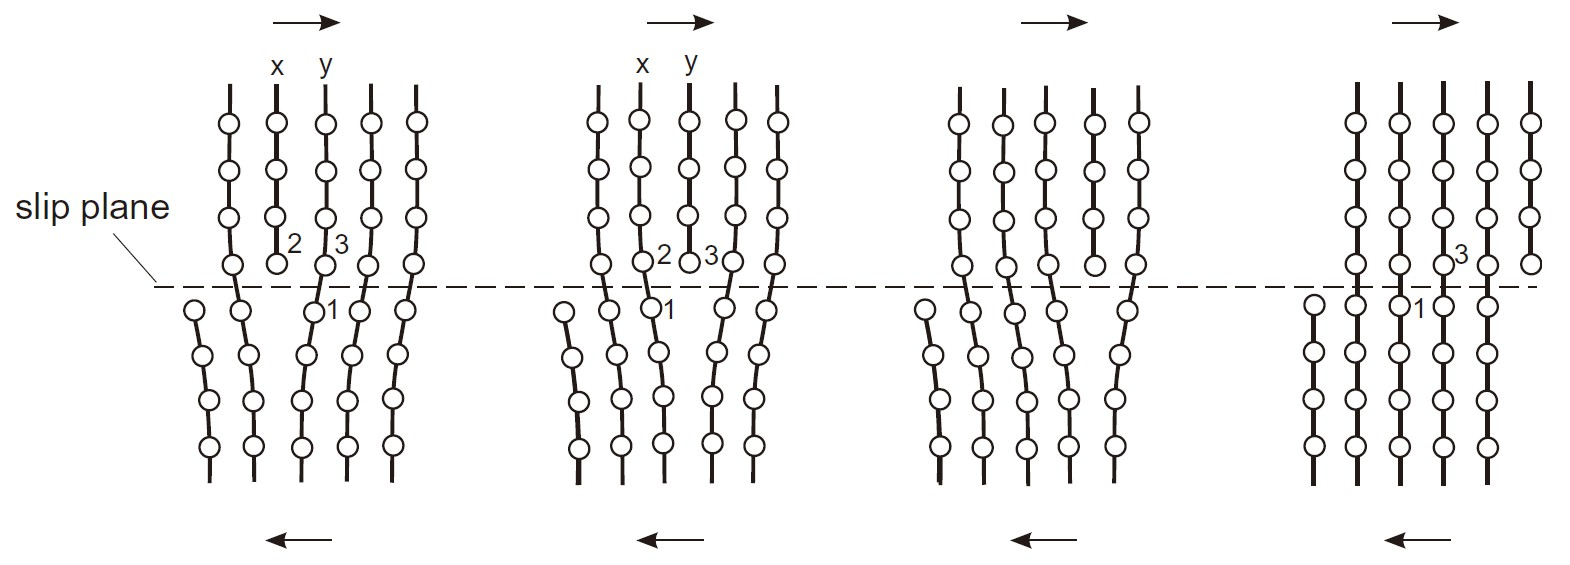
\includegraphics[width=0.7\textwidth]{fig/movement_of_edge_dislocation.jpg}
                    \caption{刃型位错滑移时周围原子的动作。}
                    \label{刃型位错滑移时周围原子的动作}
                \end{figure}
                
                从\autoref{刃型位错滑移时周围原子的动作}中可以看出,位错周围的原子只要发生微小的位移就可以造成
                位错的滑移,且位错的滑移不需要物质的长程迁移,所以位错运动传递的是一个组态,也就是原子错排的组态,
                而且滑移过程中位错的运动方向与位错线方向垂直,与位错的正负号无关,刃型位错在切应力方向运动,晶体
                上出现的台阶与位错线是平行的。

                研究发现,晶体中密排面上的位错易于滑动,这与密排面的晶面间距大,点阵阻力小有关。对于螺型位错,其
                滑移过程如\autoref{螺型位错滑移示意图}所示。螺位错周围的原子如\autoref{螺位错滑移时位错周围原子的动作}
                所示,同样只要位错周围的原子发生微调,位错就会发生滑移,而且位错的运动方向与位错线垂直,但是位错
                线移动方向与切应力垂直,这一点与刃位错不同。晶体上出现的台阶与位错线是垂直的。
                \begin{figure}[ht]
                    \centering
                    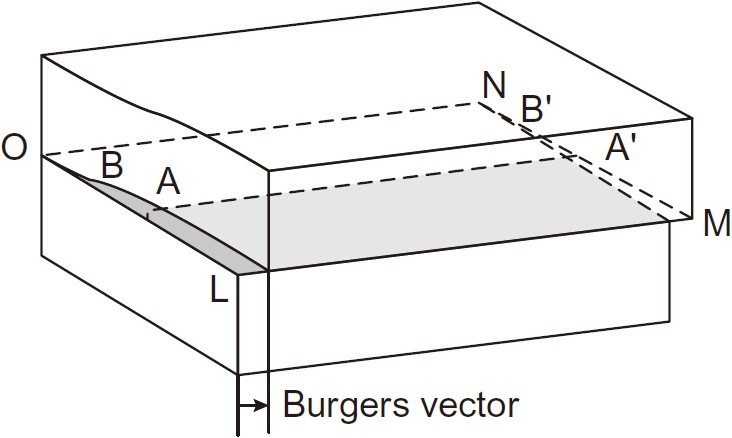
\includegraphics[width=0.5\textwidth]{fig/movement_of_screw_dislocation.jpg}
                    \caption{螺型位错从$AA'$运动到$BB'$示意图。}
                    \label{螺型位错滑移示意图}
                \end{figure}
                \begin{figure}[ht]
                    \centering
                    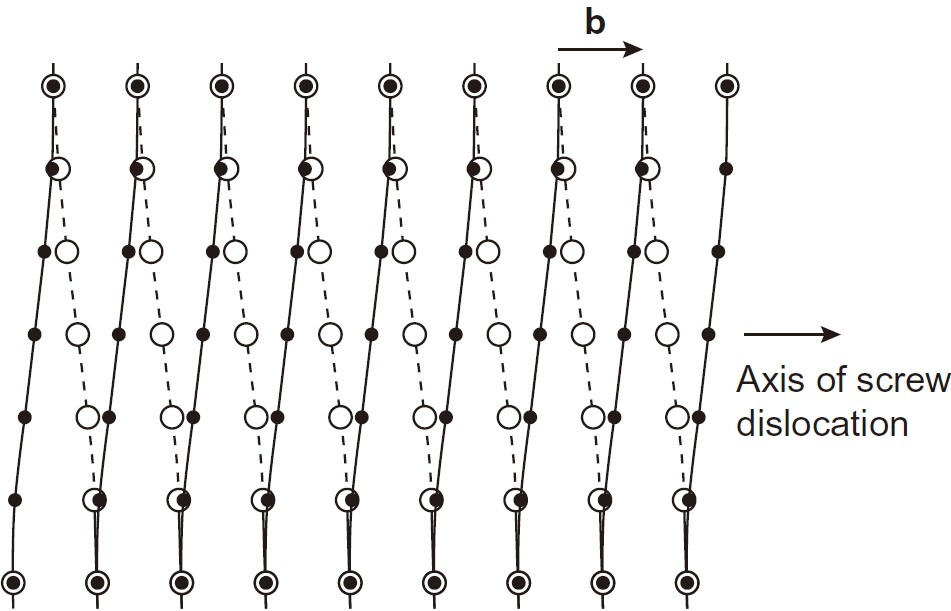
\includegraphics[width=0.5\textwidth]{fig/Arrangement_of_atoms_of_slip_of_screw_dislocation.jpg}
                    \caption{螺位错滑移时位错周围原子的动作。}
                    \label{螺位错滑移时位错周围原子的动作}
                \end{figure}

                对于混合位错,可以分解为螺位错和刃位错,因此运动方向也是两者的矢量合成方向。

                总而言之,位错的滑移过程是一个组态的传递,实际晶体中的位错滑出晶体后会在晶体表面造成台阶。
                对于位错的滑移可以得出以下结论:
                \begin{itemize}
                    \item 原子的迁移很小、所需要的力也很小,逐步推移、力在柏式矢量方向上要有分量;
                    \item 晶体错动$\vec{b}$后晶体内不存在畸变,与位错线的形状无关;
                    \item 移动方向不是由柏式矢量方向确定,而是永远与位错线垂直的方向,对于弯曲的位错线则沿其对应点的法线方向;
                    \item 刃型位错与螺型位错的滑移面、滑移方向、和台阶方向如\autoref{位错的滑移过程总结}所示。
                \end{itemize}

                \begin{table}[ht]
                    \centering
                    \caption{位错的滑移过程总结。}
                    \label{位错的滑移过程总结}
                    \begin{tabular}{@{}cccc@{}}
                        \toprule
                        位错类型 & 滑移面法线方向                & 滑移方向     & 台阶方向     \\ \midrule
                        刃位错  & $\vec{b}\times\vec{l}$ & 平行于切应力方向 & 平行位错线方向  \\
                        螺位错  & 密排面法线方向                & 垂直于切应力方向 & 垂直位错线方向 \\ \bottomrule
                    \end{tabular}
                \end{table}

                另外,刃型位错还存在一种特有的运动方式,也就是攀移。刃型位错本身如果垂直于它的滑移面运动,
                刃型位错的半薄片材料不是增长就是缩短,要实现这种运动,就需要原子的迁移来扩散质量。
                例如空位不断扩散到刃型位错,它的半薄片材料上的原子跳入空位,是的半薄片材料本身减缩,结果使
                刃型位错向上攀移一个原子间距。

                攀移的机制虽然也可以通过间隙原子的扩散,但是空位机制更为可能。攀移过程有原子的减少和增加,这
                与扩散有直接的关系,同时也与温度有关系,因为这是一个热激活过程,且其中存在体积变化,如果位错
                线不是整体攀移,还会造成割阶,如\autoref{刃型位错上的割阶}所示。
                \begin{figure}[ht]
                    \centering
                    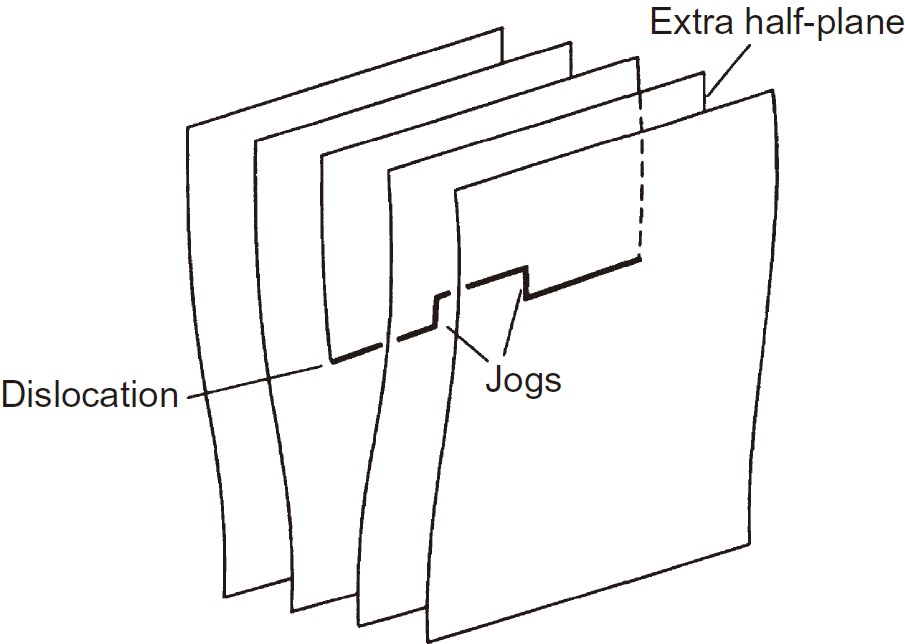
\includegraphics[width=0.5\textwidth]{fig/A_pair_of_jogs_on_an_edge.jpg}
                    \caption{刃型位错上的割阶。}
                    \label{刃型位错上的割阶}
                \end{figure}

            \subsection{位错运动与晶体变形}
            当位错滑出晶体后,会在晶体表面造成台阶,如果若干个位错滑出晶体,将会引
            起晶体的宏观变形,下面来分析一下晶体的宏观变形与位错滑移之间的关系。首先看
            一下单个位错的情况。如\autoref{刃型位错滑移造成的范型变形}所示,多个位错可以先
            叠加为一个位错$\vec{D}$。假设位错划过整个晶体扫过的面积为
            \begin{equation}
                A=l\cdot d,
            \end{equation}
            引起的变形为:
            \begin{equation}
                \gamma=\frac{D}{h}.
            \end{equation}
            如果位错只滑动了$\alpha d$,$0<\alpha<1$,位错扫过的面积为
            \begin{equation}
                A^\prime=\alpha l_2l_3,
            \end{equation}
            引起的变形为:
            \begin{equation}
                \gamma^\prime=\frac{\alpha D}{h}=\alpha\gamma.                
            \end{equation}
            \begin{figure}[ht]
                \centering
                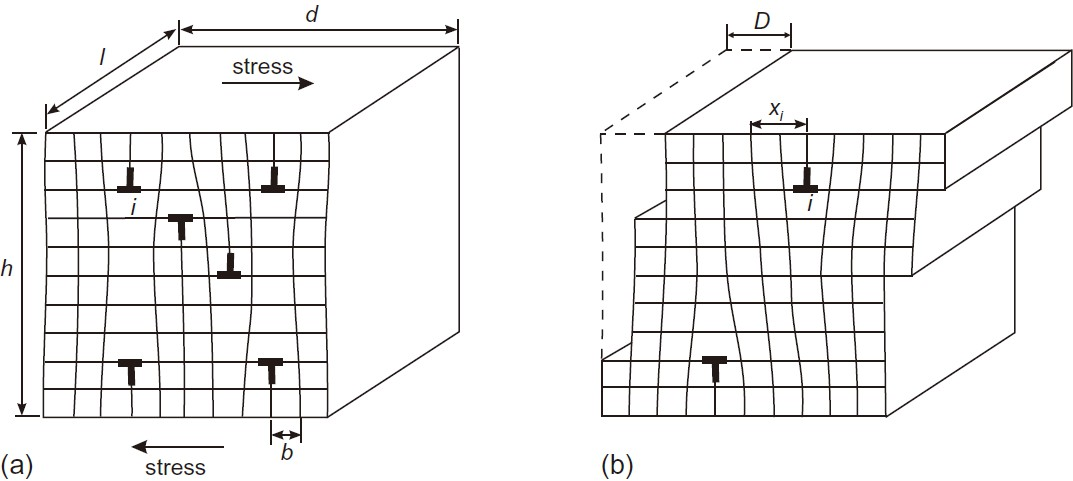
\includegraphics[width=0.7\textwidth]{fig/deformation_by_edge_dislocation.jpg}
                \caption{刃型位错滑移造成的范型变形。}
                \label{刃型位错滑移造成的范型变形}
            \end{figure}

            对于多个位错,采用面密度\index{位错!面密度}和体密度\index{位错!体密度}的方法来分析。面密度定义为
            单位面积上位错的露头数,而体密度定义为单位体积内位错的长度。因此如果若干个位错总长度为$L=\sum l_i$,
            平均移动距离为$S$,则扫过的总面积为$\sum l_i S=L\cdot S$,每根位错的平均滑移量为$\frac{L\cdot S}{A}\cdot D$,
            引起的总应变为
            \begin{equation}
                \gamma=\frac{LSD}{Ah}=\frac{LSD}{V}=\rho_v SD\label{刃型位错变形与体密度关系},
            \end{equation}
            其中$\rho_v$为位错的体密度,$V$为晶体体积,对于长方体的晶体可以也可有以下写法:
            \begin{equation}
                V=h(\cdot l\cdot d)=l\cdot(h\cdot d),
            \end{equation}
            代入\autoref{刃型位错变形与体密度关系},可得
            \begin{equation}
                \gamma=\frac{LSD}{V}=\frac{nl SD}{V}=\rho_s SD,
            \end{equation}
            其中$\rho_s$为位错的面密度。

            由于实际中位错的柏式矢量一般用$\vec{b}$表示,这里为了不产生冲突,才使用了$\vec{D}$,
            在之后的内容中,这一公式都会写作
            \begin{equation}
                \gamma=\rho Sb.
            \end{equation}

            由于刃位错在厚度方向分布不均匀,晶体会发生弯曲,如\autoref{晶体的范性弯曲}所示,上下两端弧的
            长度差为
            \begin{equation}
                \mathrm{AB}-\mathrm{CD}=(r+d)\theta-r\theta=\theta d,
            \end{equation}
            则晶体中的上半原子面数也就是位错数为
            \begin{equation}
                n=\frac{\theta d}{b},
            \end{equation}
            当晶体的厚度为$l_3$时,位错的体密度和面密度为
            \begin{align}
                \rho_v=\frac{\theta dl_3}{bV}=\frac{\theta dl_3}{b\theta rdl}=\frac{1}{br},\\
                \rho_s=\frac{\theta d}{b\theta rd}=\frac{1}{br}=\rho_v.
            \end{align}
            \begin{figure}[ht]
                \centering
                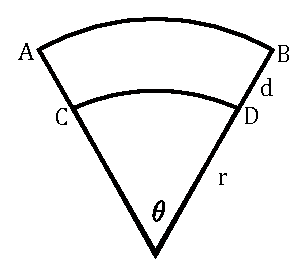
\includegraphics[width=0.5\textwidth]{fig/bending_of_crystal_for_dislocation.eps}
                \caption{晶体的范性弯曲。}
                \label{晶体的范性弯曲}
            \end{figure}

            \subsection{作用在位错上的力}
                在\autoref{subsection:点阵阻力}中,将点阵阻力定义为原子势的梯度,在这一节中,
                仍然使用这个定义,
                \begin{equation}
                    F=-\nabla U\label{位错力的定义},
                \end{equation}
                并用其分析位错运动中受到的滑移力、攀移力等。
                
                \subsubsection{滑移力}
                    假设位错的滑移面面积为$S$,位错线长度为$\xi$,滑动了$\dif l$,
                    位错的柏式矢量为$\vec{b}$,扫过的面积为$\xi\cdot\dif l$,产生的平均滑移量为
                    \begin{equation}
                        A=\frac{\xi\dif l}{S}\cdot b=\alpha b,
                    \end{equation}
                    滑移面受到的外力为
                    \begin{equation}
                        F=S\cdot\tau,
                    \end{equation}
                    外力所做的功为
                    \begin{equation}
                        \dif W=F\cdot A=\frac{S\tau b\xi\dif l}{S}=\tau bd\xi\dif l=\dif U,
                    \end{equation}
                    根据定义\autoref{位错力的定义}可得
                    \begin{equation}
                        F^{\prime}=\frac{\dif U}{\dif l}=\tau b\xi,
                    \end{equation}
                    令$\xi=1$,则有
                    \begin{equation}
                        F^{\prime}=\tau b.
                    \end{equation}

                    位错受到的滑移力有以下特点
                    \begin{itemize}
                        \item 力的方向垂直于位错线;
                        \item $\tau$必须在柏式矢量方向上有分量;
                        \item 滑移力为组态力,并不是位错附近原子实际受到的力。
                    \end{itemize}
                \subsubsection{攀移力}
                    假设一小部分的位错线$l$沿半原子面方向发生位移$s$,此时发生的体积变化为
                    \begin{equation}
                        \dif V=b\cdot l\times s=s\cdot b\times l,
                    \end{equation}
                    面积微元为$\dif S=\dif V/s$,受力为
                    \begin{equation}
                        F=\sigma_{yy}\dif S,
                    \end{equation}
                    发生攀移所做的功为
                    \begin{equation}
                        \dif W=F\cdot s=\sigma_{yy} s\dif S=\sigma_{yy}slb,
                    \end{equation}
                    假设位错的攀移力为$F_c$,此过程中做功为
                    \begin{equation}
                        \dif W=F_c\cdot l\cdot s,
                    \end{equation}
                    所以位错的攀移力为
                    \begin{equation}
                        F_c=-\sigma_{yy}\cdot b.
                    \end{equation}
                    
                    这一过程需要扩散,因此也需要热激活,因此攀移一般发生在较高的温度下。
                \subsection{位错攀移阻力和化学力}
                    假设一个原子所占的体积为$\Omega$,则填补$\dif V$的空隙需要$\dif V/\Omega$个
                    点缺陷,假设$\Omega=b^3$,所以原子数为
                    \begin{equation}
                        \dif n=\frac{ls}{b^2}.
                    \end{equation}

                    假设攀移阻力为$F_z$,则攀移形成体积$\dif V$所需的功为
                    \begin{equation}
                        W=\sigma_{yy}\cdot\dif V,
                    \end{equation}
                    需要的原子数为$\dif n=\dif V/\Omega$。

                    假设点缺陷形成能为$E_f$,则填补$\dif V$的形成能为
                    \begin{equation}
                        \dif n\cdot E_F=\frac{E_f ls}{b^2}=F_z\cdot s=-\sigma_{yy}lsb,
                    \end{equation}
                    因此有
                    \begin{equation}
                        F_z=\frac{E_f}{b^2}=-\sigma_{yy}b,
                    \end{equation}
                    因此空位形成能与应力的关系为
                    \begin{equation}
                        \sigma_{yy}=\frac{E_f}{b^3},
                    \end{equation}
                    一般来讲,空位形成能为
                    \begin{equation}
                        E_f=\frac{\mu b^3}{5}.
                    \end{equation}

                    如果晶体中存在过饱和空位,这时单位时间内体哦啊到位错上的空位数
                    就要超过离开的位错数,从而产生位错攀移的驱动力,这种里称为化学力。
                    假设在某一温度下,晶体的空位平衡浓度为$c_v$,而实际浓度为$c$,则空位的化学势,即
                    与一个空位消失与位错相关的自由能变化为
                    \begin{equation}
                        \mu_v=\frac{\partial F}{\partial n}=kT\ln\frac{c}{c_0},
                    \end{equation}
                    单位为错攀移单位距离时,所需的空位数为$1/b^2$,相应的自由能变化就被
                    定义为单位长度位错线所受的化学攀移力,即
                    \begin{equation}
                        F_c=\frac{1}{b^2}kT\ln\frac{c}{c_0}.
                    \end{equation}
                \subsection{位错的一般力公式}
                    $\dif l$的位错受到空间力场$\sigma$的作用,在滑移面A上运动$\dif s$
                    距离,此时的滑移面积为$\dif A=\dif l\cdot\dif s$。设$\vec{n}$为A面法线,
                    对应矢量为$(n_x,n_y,n_z)$,空间中一个面积元为
                    \begin{equation}
                        \dif A =n \cdot\dif A.
                    \end{equation}
                    
                    空间中的应力场包括三个正应力、六个切应力,用应力张量表示
                    \begin{equation}
                        \sigma=\begin{bmatrix}
                            \sigma_{xx}&\tau_{xy}&\tau_{xz}\\
                            \tau_{yx}&\sigma_{yy}&\tau_{yz}\\
                            \tau_{zx}&\tau_{zy}&\sigma_{zz}
                        \end{bmatrix}.
                    \end{equation}
                    则空间中任意斜面的总外力为
                    \begin{equation}
                        F=\sigma\cdot n\dif A,
                    \end{equation}
                    外力使该面移动b所做的功为
                    \begin{equation}
                        W=b\cdot\left( \sigma\cdot n\dif A \right)=b\left[ \sigma\cdot(\dif l\times\dif s) \right]\cdot\dif s,
                    \end{equation}
                    根据矢量叉乘的性质可以变成
                    \begin{equation}
                        W=\left( b\sigma\times\dif l \right)\dif s,
                    \end{equation}
                    设作用在位错上的力为$\dif F$,滑移矢量为$\dif s$,柏式矢量为$\vec{b}$,
                    则$\dif F$做功为
                    \begin{equation}
                        W=\dif F\cdot\dif s=\left( b\sigma\times\dif l \right)\dif s,
                    \end{equation}
                    因此
                    \begin{equation}
                        \dif F=b\sigma\times\dif l,
                    \end{equation}
                    如果令$t$为$\dif l$的单位向量,则可以写为
                    \begin{equation}
                        \dif F=b\sigma\times t.
                    \end{equation}
                    所以位错运动受力的特点为:
                    \begin{itemize}
                        \item[1] 受力方向总与位错线垂直;
                        \item[2] 位错受力与外力方向不一致。
                    \end{itemize}
                \subsection{位错像力}
                    在研究半无限大介质中的一个位错时,这个位错和介质的表面平行,距离表面的距离为$l$,
                    根据位错应力场计算的结果在表面存在应力,但是实际上表面的总应力应当为零,这就需要在
                    以表面为对称的位置上存在一个想象的柏式矢量相反的位错,这样才能满足边界条件。

                    实际上产生这项吸引力的原因是位错倾向于接近自由表面以松弛其弹性应变能。
                    按照组态力的概念我们用一个力来描述系统自由能降低的趋势,这个力就是像力。
                    更为具体的分析结果可以通过\href{https://brilliant.org/wiki/greens-functions-in-physics/}{Green函数}来分析。
        \section{位错与晶体缺陷间的相互作用}
            由于晶体中的位错具有长程应力场,当晶体中同时存在有其他晶体缺陷时,同样
            地这些缺陷改变了原子的规则排列,从而在晶体中引入了畸变,它们之间就会发生相
            互作用。本节主要讨论位错与其它位错以及点缺陷之间的相互作用。
            
            晶体之间存在大量的位错,因此,各个位错之间会由于应力场的作用产生相互长程应力
            作用,当两个位错相遇时,两者之间还会产生短程的相互作用。首先来分析长程应力场
            之间的相互作用。
            \subsection{弹性应力场之间的相互作用}
                    晶体中常常包含有很多位错,它们的弹性应力场之间发生干涉和相互作用,
                    并且将影响到位错的分布和运动。直接处理任意分布大量位错之间的相互作用是
                    非常困难的,有效的方法是从最简单、最基本的情况入手。

                    首先讨论一堆螺位错之间的相互作用,在坐标原点和$(r,\theta)$处有一对平行于
                    $z$轴的同号螺型位错,柏式矢量分别为$\vec{b}_1$和$\vec{b}_2$。位错$\vec{b}_1$
                    在$(r,\theta)$处的应力场为
                    \begin{equation}
                        \sigma_{\theta,z}=\frac{\mu b_1}{2\pi r},
                    \end{equation}
                    对于位错$\vec{b}_2$来说,此应力分量作用在它的滑移面上且平行于它的柏式矢量,即
                    ,满足滑移的条件,按照滑移力的计算,位错$\vec{b}_2$受到的力为
                    \begin{equation}
                        F=\frac{\mu b_1 b_2}{2\pi r}\label{两个螺型位错之间的作用力},    
                    \end{equation}
                    这个力要求它沿两位错连线方向向往外运动,里的大小随两位错间距的增加而降低。
                    同理,$\vec{b}_1$也受到$\vec{b}_2$大小相等方向相反的力。如果俩个螺位错的符号相反,
                    则就会变为吸引力,这与两条通电导线的作用相似。
                    
                    对于平行滑移面两个刃型位错,两者的位错线与$z$轴平行,柏式矢量分别为$\vec{b}_1$和$\vec{b}_2$。
                    根据\autoref{刃位错的x主应力}和\autoref{刃位错的切应力},$\vec{b}_2$所在处$\sigma_{xx}$使
                    其受到攀移力,$\tau_{yx}$使位错$\vec{b}_2$受到滑移力,分别为
                    \begin{align}
                        F_x&=\sigma_{yx}b_2=\frac{\mu b_1b_2}{2\pi(1-v)}=\frac{z(x^2-y^2)}{(x^2+y^2)^2}\label{两个刃型位错之间的相互作用力},\\
                        F_y&=-\sigma_{xx}b_2=\frac{\mu b_1b_2}{2\pi(1-v)}=\frac{y(3x^2+y^2)}{(x^2+y^2)^2}.
                    \end{align}

                    对得到的结果分析可知,$F_y$与$y$同号,也就是当位错$\vec{b}_2$在位错$\vec{b}_1$滑移面
                    上边时,受到的攀移力$F_y$指向上,在滑移面下边时,受到的攀移力指向下,所以沿$y$轴方向两
                    位错是互相排斥的。然而当$x^2<y^2$时$F_x$指向外,所以两位错沿$x$方向相互排斥,当$x^2<y^2$
                    时,$F_x$指向内,所以两位错沿$x$轴方向互相吸引,如\autoref{两刃型位错在x轴方向上的相互作用}
                    所示。在$x=0$以及$x=\pm y$的位置,$F_x$虽然等于零,但是这两种位置不同。$x=0$为稳定平衡位置,
                    \begin{figure}[ht]
                        \centering
                        \includegraphics[width=0.5\textwidth]{fig/force_of_edge_dislocations_along_x_axis.eps}
                        \caption{两同号刃型位错在$x$轴方向上的相互作用。}
                        \label{两刃型位错在x轴方向上的相互作用}
                    \end{figure}
                    因为当位错$\vec{b}_2$稍微偏离这个位置时,会受到回复的力,而$x=\pm y$是不平衡位置,
                    $\vec{b}_2$发生偏离时,受到的力使其偏离的更远。所以相同符号的刃型位错沿着
                    与它们柏式矢量相垂直的方向排列起来是稳定的\footnote{这样的位错排列会形成一种晶粒边界。}。
                    加入两个位错的符号相反,它们之间的作用力的方向也要改变,而$x=0$变为不稳定的平衡位置,
                    $x=\pm y$变为稳定的平衡位置。符号相反的两个位错依靠弹性相互作用在\ang{45}方向上彼此
                    束缚在一起,构成通常所围的位错偶极子。

                    当两个位错相互平行,分别为纯螺型和纯刃型,由于螺位错的应力场没有使刃位错受力的应力分量,
                    刃位错的应力场也没有使螺位错受力的应力分量,所以两个位错没有相互作用。

                    对于具有任意柏式矢量的两个平行的直线位错,可以把每个位错都分解为刃型分量和螺型分量,
                    然后依次计算两个螺型分量和两个刃型分量之间的相互作用,并且叠加起来,就得到了任意两个
                    位错之间的相互作用,对所得记过可以近似地归纳为:若柏式矢量夹角小于$\frac{\pi}{2}$,
                    则两个位错互相排斥,若柏式矢量夹角大于$\frac{\pi}{2}$,则两个位错互相吸引。
            \subsection{位错塞积}
                现在我们开始研究位错集群在外加应力、障碍以及集群内部的相互作用力下的平衡问题。晶体材料中通常有许多位错,
                在外加应力作用下在滑移面上滑动。假如滑移面上遇到强的障碍物,
                领先的位错不能越过障碍,这样就会形成由许多位错组成的塞积群。
                实际材料中的晶界或第二相硬颗粒都是可以产生位错塞积群的障碍物。

                在分切应力作用下,由同一位错源放出的位错在障碍前受到阻碍,这些位错就在障碍前排列起来,
                这种位错组态称为塞积群,如\autoref{实际晶体中的塞积群}所示。

                位错塞积群在受力上可以分为三类:
                \begin{itemize}
                    \item[1] 领先位错受到的障碍物的作用;
                    \item[2] 各个位错之间的相互作用;
                    \item[3] 外加应力作用。
                \end{itemize}

                对于外力具体的求解过程比较复杂,这里只给出主要结果。领先位错前的切应力
                为
                \begin{equation}
                    \tau^{\prime}=n\tau,
                \end{equation}
                此式表明,当有$n$个位错被外加切应力$\tau$推向障碍物时,位错塞积群的前端将
                产生$n$倍与外力的应力集中。

                塞积群的长度为
                \begin{equation}
                    L=xn=\frac{\vert A\vert \pi^2}{8n\tau}(n-1)^2,
                \end{equation}
                与切应力$\tau$成反比。
                \begin{figure}[ht]
                    \centering
                    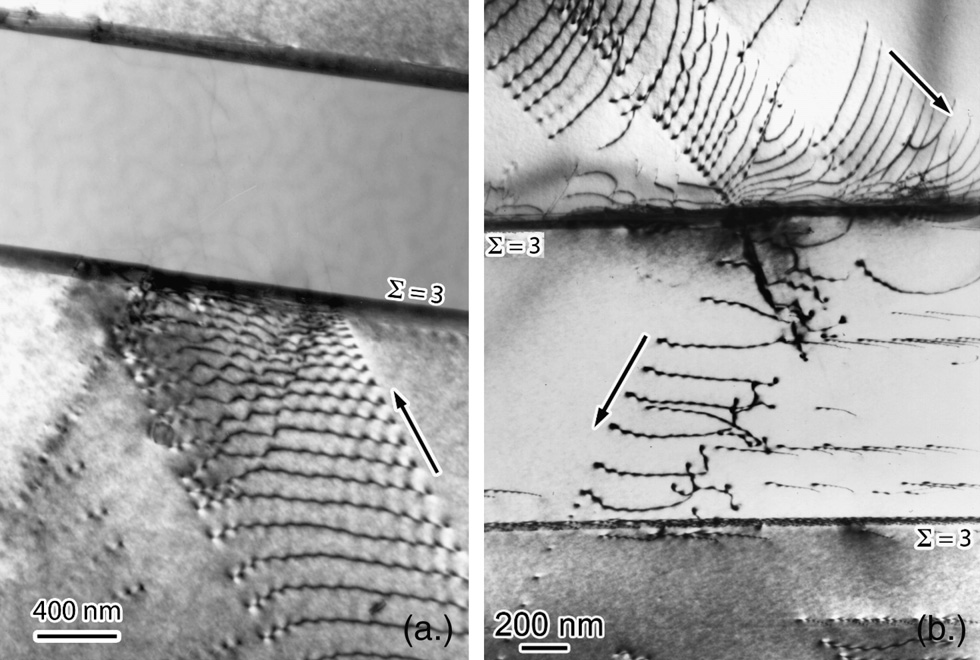
\includegraphics[width=0.7\textwidth]{fig/pile_up_groups_&_slip_transmit_twin_boundary.jpg}
                    \caption{层错能较低的材料的孪晶界的TEM原位照片\cite{SANGID2011283},(a)为滑移被孪晶界阻碍,形成位错塞积群,(b)为加载力过大时,滑移进入孪晶界。}
                    \label{实际晶体中的塞积群}
                \end{figure}
            
            \subsection{位错交割}
                在晶体的范性形变过程中会产生不同滑移面上位错相交截的现象.这里牵涉到位
                错间的弹性相互作用以及近程相互作用。下面分别考虑这两种相互作用:
                \begin{itemize}
                    \item[1] 弹性相互作用:设不同滑移面上的位错线相交,且夹角大于$\frac{\pi}{2}$,由于弹性相互作用,两个位错可以合成新的位错线段,以降低弹性能;
                    \item[2] 位错的中心区可能产生近程的相互作用。
                \end{itemize}

                对于在滑移面上运动的位错来说,穿过此滑移面的其它位错称为林位错\index{林位错}。
                林位错会阻碍位错的运动,但是若应力足够大,滑动的位错将切过林位错继续前进。位错相互切割的过程称为位错交割\index{位错交割}。

                \begin{figure}[ht]
                    \centering
                    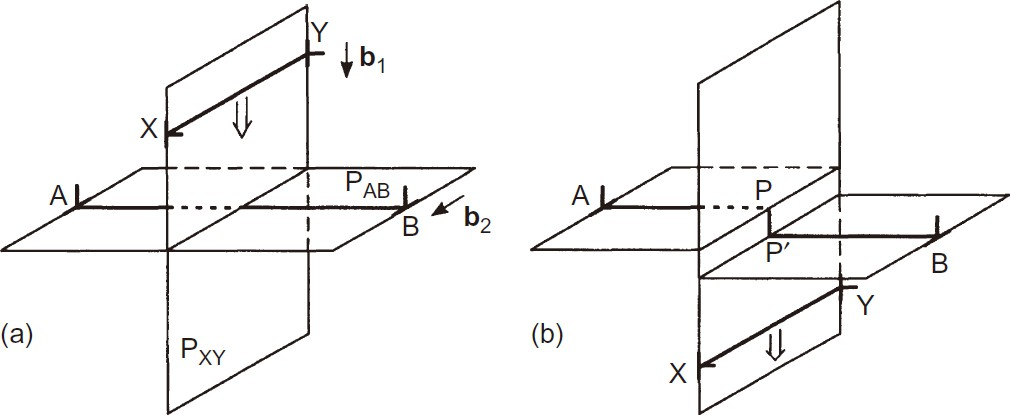
\includegraphics[width=0.7\textwidth]{fig/Intersection_of_edge_dislocations_with_Burgers_vectors_at_right_angles_to_each_other.jpg}
                    \caption{两个柏式矢量垂直的刃位错的相互作用\cite{HULL2011137},(a)位错xy沿滑移面$P_{\mathrm{xy}}$移动,并切过$P_{\mathrm{AB}}$面的AB位错,(b)为
                        xy已经切过AB,并且产生了$\mathrm{PP}^{\prime}$割阶。}
                    \label{两个垂直的刃位错的相互作用}
                \end{figure}
                
                \autoref{两个垂直的刃位错的相互作用}表示两个刃位错的相互交割,$\mathrm{P}_{\mathrm{AB}}$面
                的位错保持不动,而$\mathrm{P}_{\mathrm{xy}}$面的位错向下移动,柏式矢量为$\vec{b}_1$,当$\vec{b}_1$
                扫过时$\mathrm{P}_{\mathrm{AB}}$面两侧发生了相对位移$\mathrm{PP}^{\prime}$,方向和大小与
                取决于$\vec{b}_1$。由于位错的连续性,即位错不能在晶体内部中断,$\mathrm{PP}^{\prime}$必然是
                一小段位错,又由于柏式矢量的守恒性,它的柏式矢量也必然是$\vec{b}_2$。这一小段位错$\mathrm{PP}^{\prime}$
                称为位错割阶。产生割阶需要能量供给,所以交割过程对位错运动是一种阻碍。粗略估计,
                割阶能量的数量级为$\frac{\mu b^3}{10}$,对于一般金属约等于十分之几个电子伏特。

                其次考虑一个刃型位错与一个螺型为位错的交割,如\autoref{刃型位错与螺型位错交割}所示,图中螺型位错的柏式矢量为
                $\vec{b}_2$,按照螺型位错的特点,被它贯穿的一组晶面组成一个螺旋面。另一个位错的柏式矢量为$\vec{b}_1$,
                是一个刃型位错,其滑移面恰好是螺型位错$\vec{b}_2$的螺旋面。当位错$\vec{b}_1$切过螺型位错后,
                变成了分别位于两层晶面上的两段位错,两者的连线$\mathrm{PP}^{\prime}$也是一个位错割阶,大小
                个方向等于螺型位错的柏式矢量$\vec{b}_2$,而其自身的柏式矢量与刃型位错相同,仍然是一段刃型位错,
                割阶随位错$\vec{b}_1$一同向前的运动也是滑移。
                \begin{figure}[ht]
                    \centering
                    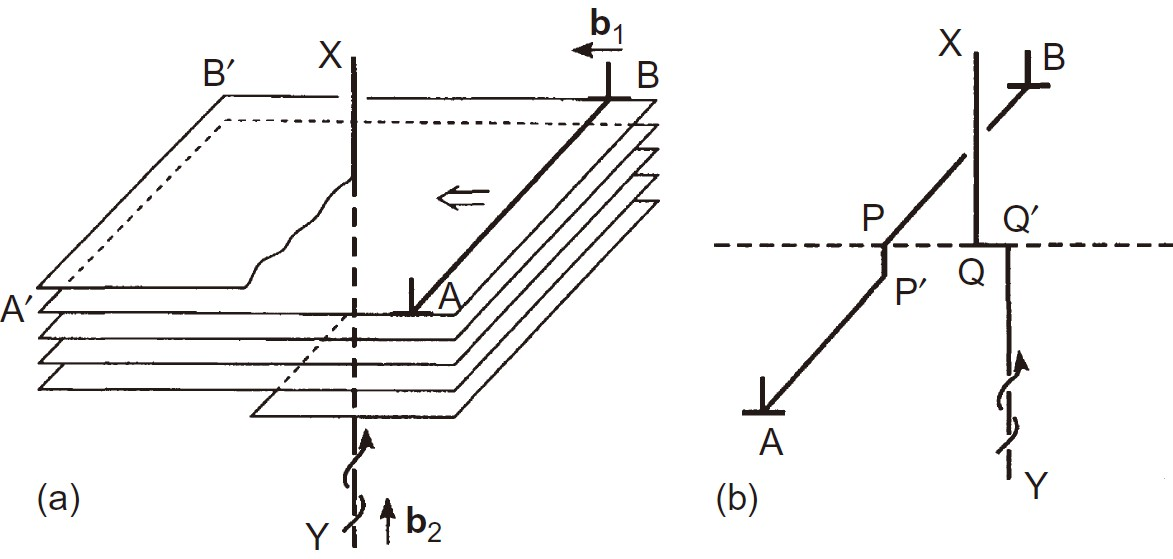
\includegraphics[width=0.7\textwidth]{fig/Intersection_of_an_edge_dislocation_with_a_right-handed_screw_dislocation.jpg}
                    \caption{刃型位错$\mathrm{AB}$与垂直的右螺型位错$\mathrm{XY}$的相互作用,(a)$\mathrm{AB}$在滑移面移动切割$\mathrm{XY}$,
                        由于螺位错使晶体螺旋上升一层,因此当切过螺位错,到达$\mathrm{A}^{\prime}\mathrm{B}^{\prime}$时,$\mathrm{AB}$不再处于
                        同一个平面,也就是在(b)中的割阶$\mathrm{PP}^{\prime}$。}
                    \label{刃型位错与螺型位错交割}
                \end{figure}

                一般情况下,两个位错交割时,每个位错上都要产生一小段位错,它们的柏式矢量与其本身相同,但是
                大小和方向取决于另一位错的柏式矢量。当交割产生的小段位错不在所属的位错的滑移面时,则称为位错割阶,且所有的割阶都是刃型位错,
                如果小段位错位于所属位错的滑移面上,则相当于位错扭折\index{位错扭折}。

            \subsection{位错与溶质原子之间的相互作用}
                \subsubsection{弹性交互作用}
                    由于位错具有长程应力场,因此可以与溶质原子产生的畸变发生相互作用,这种作用称为弹性交互作用。

                    对于刃型位错来说,假设以位错核心为原点建立极坐标系,假设晶体中的一个基体原子的半径为$r_0$,
                    在$(r,\theta)$存在一个半径为$r_0(1+\varepsilon)$的小球,相当于将一个体积与基体原子不同的
                    溶质原子放入晶体的空位,其中$\varepsilon$称为错配度,表示溶质原子与基本原子的差别的大小。
                    在此过程中,外力反馈位错应力场所作的共就是位错与溶质原子的交互作用能。由于小球在周围介质中
                    引起的位移垂直于球面,位错的应力场中只有正应力分量$\sigma_{xx}$,$\sigma_{yy}$和$\sigma_{zz}$
                    做功,平均值为
                    \begin{equation}
                        \sigma=\frac{1}{2}\left( \sigma_{xx}+\sigma_{yy}+\sigma_{zz} \right),
                    \end{equation}
                    在位移$\varepsilon a$的过程中,位错应力场所做的功为$4\pi\sigma\varepsilon r_0^3=\sigma\Delta V$,
                    $\Delta V=4\pi\varepsilon r_0^3$为溶质原子与基体原子的体积差。从而位错与溶质原子的相互作用能为
                    \begin{equation}
                        U=-\frac{1}{2}\left( \sigma_{xx}+\sigma_{yy}+\sigma_{zz} \right)\Delta V,
                    \end{equation}
                    把刃型位错应力场\autoref{刃位错的x主应力}、\autoref{刃位错的y主应力}和\autoref{刃位错的z主应力}代入上式,得到
                    \begin{equation}
                        U=A\cdot\frac{\sin\theta}{r},A=\frac{\mu b}{3\pi}\frac{1+v}{1-v}\Delta V,
                    \end{equation}
                    其中$r$和$\theta$代表溶质原子的坐标位置。

                    上式表明,当$\Delta V>0$,在$0<\theta<\pi$处,$U$为正,在$\pi<\theta<2\pi$处,$U$
                    为负。当$\Delta V<0$时则相反。平衡状态要求相互作用能最小,所以,比集体原子大的置换式溶质
                    原子和间隙原子将被位错的压缩区排斥,被位错的膨胀区吸引,而比基体原子小的置换式溶质原子和
                    空位的移动趋势恰好相反。

                    由于溶质原子与位错有相互作用,若时间和温度允许,它们将向位错附近聚集,形成科垂耳气团\index{科垂耳气团},
                    使位错的运动受到限制。因为在这种情况下,推动位错运动,或者首先挣脱气团的束缚,或者拖着气团一起前行,
                    无论如何都要做更多的功,这对应着拉伸曲线中的上屈服点。

                    对于螺位错来说,则没有弹性相互作用,这是因为螺位错的应力场只有切应力分量,二溶质原子产生的畸变又被
                    假定为球形对称,但是一旦畸变不再是球形,螺位错也会与溶质原子发生相互作用\footnote{比如体心立方铁晶格中的碳原子或氮原子。}。
                    这种相互作用有时称为史诺克气团\index{史诺克气团}。

                \subsubsection{模量相互作用}
                    设溶质原于大小和基体原于基本一样,但它的弹性不同,由此而产生的交互作用就是模量交互作用。
                    我们在这里仅做定性的分析。首先假定溶质原子比基体硬一些,即切变模量大一些。当一个螺型位错移近这个“硬点”的时候,
                    通过它的切应力对这个硬点施以变形的功不同于没有这个硬点而为基体时的变形功。
                    这个功的差额就是模量交互作用能的量度。在极端情况下,设溶质原子很硬,很难变形,
                    这种原子将抗拒螺型位错向它移近;若溶质原子比基体软一些,情况相反,
                    原子倾向于靠近位错,位错由这个软点拉出去,需要额外的功。刃型位错和螺形位错不同,
                    前者除了它的切应力对溶质原子施加切变以外,还可以通过它的正应力对溶质原子施加正向的变形。
                    刃型位错和溶质原子之闻也有模量交互作用。
                \subsubsection{化学相互作用}
                    以上讨论的都是全位错和溶质原子通过位错的应力场和溶质原子产生的体膨胀或畸变发生作用。现在阐述另一种不同的作用,全位错分解为不全位错,
                    ,其间有层错,在层错区溶质原子的浓度(平衡时)应该不同于基体中的溶质浓度。
                    这种作用首先被Suzuki所认识,称为化学作用。
                    当位错运动时,这种不均匀分布的溶质原子也将随位错移动,因此这种组态通常称为Suzuki气团(铃木气团)\index{铃木气团}。

        \section{位错的增殖}
            \subsection{位错起源}
                根据理论计算,位错的能量很大,除非晶体受到的应力基金理论切变强度,说明位错不是靠热激活
                能产生的,因此位错不会在晶体中均匀形核。位错出现的位置基本有以下几种:
                \begin{itemize}
                    \item 应力集中的位置可能形成位错;
                    \item 在不均匀变形中可能产生位错;
                    \item 过饱和的空位凝胶成空位片,空位片的坍塌导致位错环形成;
                    \item 杂质分凝、偏析,凝固后晶体成分与凝固之前不同,造成点阵常数不同,累计结果形成位错;
                    \item 晶体中沉淀无或夹杂无在周围基体中产生较大应力,导致位错产生;
                    \item 结晶过程中正在生长的两部分晶体相遇,如果两者的位相有轻微差别,在结合的位置就会形成位错。
                \end{itemize}
            \subsection{位错增殖}
                研究发现,退火金属的位错密度在$\SI{1e6}{\cm^{-2}}$左右,而冷变形金属的位错密度会急剧增加到
                \SI{1e12}{\cm^{-2}}左右,这说明在变形过程中存在位错密度的增殖过程,对于这一过程的解释,
                以Frank-Read 源\index{Frank-Read源}理论最为简洁。

                设想晶体中有一段位错线两端被钉住,在应力作用下,位错线由于滑移而弯曲,二位错所受
                作用力恒与位错相垂直,则位错的发展情况如\autoref{Frank-Read源}所示。
                \begin{figure}[ht]
                    \centering
                    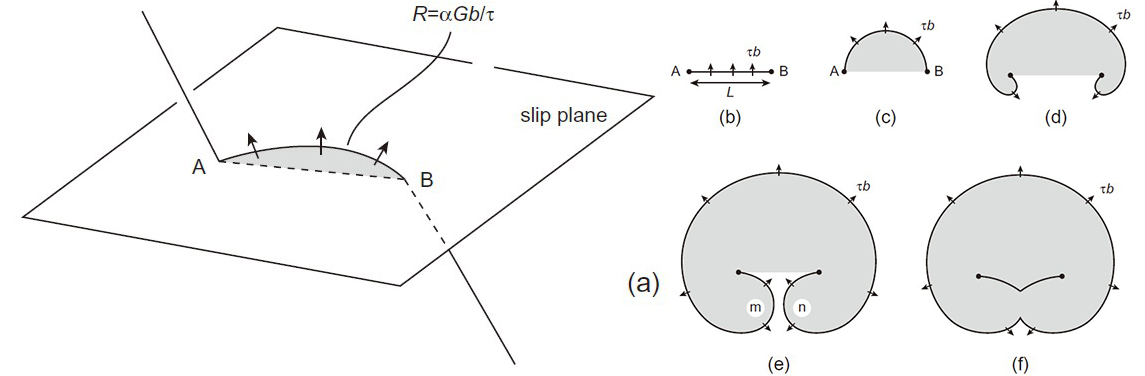
\includegraphics[width=0.8\textwidth]{fig/Frank_read_sources.jpg}
                    \caption{Frank-Read位错源图示。}
                    \label{Frank-Read源}
                \end{figure}
                当弯曲的线段相互靠近时。可以相互抵销,形成一闭合的位错圈和一段短线.这样的过程可以反复进行下去,
                源源不断地产生新的位错圈.当位错圈和晶体表面相截,就形成了台阶,这就是显微镜中所观察到的滑移线.
                当更多的位错圈和表面相交,中央部分的台阶逐渐变高,并向两侧伸展。

                下面进一步讨论为了开动位错源需要多大的应力,为此首先考虑一段弧形位错在滑移力和线张力的
                共同作用下的平衡。设想滑移面上的一端微元位错线$ab$在滑移力$F_\tau$和线张力的共同作用下到达
                平衡。平衡时,位错线$ab$的张角为$\delta\theta$,曲率半径为$R$,如\autoref{一段弧型位错的平衡}
                所示。根据静力学
                \begin{figure}[ht]
                    \centering
                    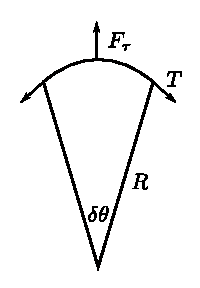
\includegraphics[scale=1]{fig/balance_of_FR_source.eps}
                    \caption{一段弧形位错的平衡。}
                    \label{一段弧型位错的平衡}
                \end{figure}
                \begin{equation}
                    2T\sin\frac{\delta\theta}{2}=F_\tau R\delta\theta,
                \end{equation}
                考虑到$\delta\theta$为无穷小,可以简化为
                \begin{equation}
                    2T\frac{\delta\theta}{2}=F_\tau R\delta\theta,
                \end{equation}
                或
                \begin{equation}
                    F_\tau=\frac{T}{R},
                \end{equation}
                将$F_\tau=\tau b$和$T=\frac{1}{2}\mu b^2$代入上式,得到
                \begin{equation}
                    \tau=\frac{\mu b}{2R}\label{线张力和切应力平衡条件},
                \end{equation}
                此式表面,当位错弧线达到平衡时,外加应力与弧线的曲率半径成反比,即位错曲率半径越小,
                要求与之相平衡的力越大。

                在\autoref{Frank-Read源}中,位错线AB弯曲之后,需要一定大小的切应力与之平衡,
                曲率约到,相平衡的切应力也越大。当位错线称为半圆形时,曲率达到了最大值,需要的切应力
                也为最大。可见,一个Frank-Read位错源受到适当切应力作用时,就开始运动和弯曲。
                起初为了弯曲能继续进行,所需的应力越来越大,直到位错完成半圆形,相应的的应力达到最大值,
                此后位错向外膨胀,曲率开始缩小,所需的应力也减小。因此位错开动的力取决于\autoref{Frank-Read源}
                中的(c)图对应的状态,此时的切应力为临界应力,\autoref{线张力和切应力平衡条件}可得临界切应力为
                \begin{equation}
                    \tau_c=\frac{\mu b}{2R}=\frac{\mu b}{l},
                \end{equation}
                其中$l$为位错线$AB$的长度,假设$l$长为\SI{1e-4}{\cm},$b$长度为\SI{1e-8}{\cm},
                对应的切应力为$10^{-4}\mu$,这和实际晶体的屈服强度接近。

                \begin{figure}[ht]
                    \centering
                    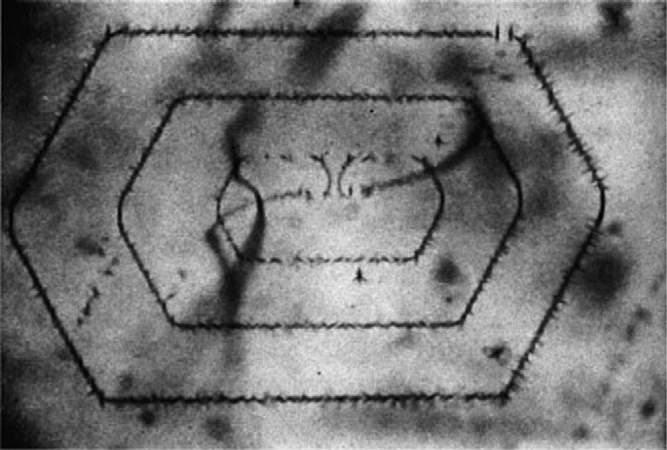
\includegraphics[width=0.7\textwidth]{fig/Frank_Read_source_in_a_silicon_crystal.jpg}
                    \caption{硅晶体中的Frank-Read位错源,通过缀饰法在硅晶体中显示出来的\cite{Dash1958}。}
                    \label{硅晶体中的Frank-Read位错源}
                \end{figure}

                \autoref{硅晶体中的Frank-Read位错源}是一个典型的位错源照片\cite{Dash1958},这个位错元正在释放位错环的时候被缀饰
                质点固定住了,由于硅是共价键晶体,错排能垒很高,所以位错线表现出明显的取向性。
        \section{实际晶体中的位错}
            前面我们讨论的位错的各种情况都是基于一个前提,以简单立方为例,而并未联
            系到晶体的具体结构,同时位错的柏氏矢量均为一个原子间距。但是在实际晶体中由
            于其具有不同的点阵类型,例如面心立方,体心立方等,其位错类型也会发生变化。
            首先我们定义全位错为柏氏矢量等于点阵矢量的位错,所以前面我们讨论的问题均是
            基于全位错\index{全位错}来考虑的。
            
                许多金属属于面心立方结构,这样的金属晶体的范性形变和晶体中的位错结构有
                密切关系,面心立方晶体中位错结构比上面经常作为例子的简单立方晶体中的位错
                复杂得多。设面心立方结构单位晶胞边长为$a$,点阵矢量$a$为$\langle110\rangle/2$类型,
                通常简写为$\frac{1}{2}\langle110\rangle$,也是最短的点阵矢量。所以面心
                立方晶体位错的柏式矢量最可能为$\frac{1}{2}\langle110\rangle$。之前证明
                位错的能量与$b^2$成正比,所以以$\frac{1}{2}\langle110\rangle$为柏式矢
                量的位错的应变能低于以$\langle100\rangle$为柏式矢量的位错能量,这就是面心立方
                结构没有$\langle100\rangle$位错的原因,而$\frac{1}{2}\langle110\rangle$为
                面心立方结构的单位位错。

                既然位错的应变能与位错的$b^2$成正比,因此一般来讲,最稳定的位错的柏式矢量应该为晶体的
                最短平移矢量。比如简单立方中的$\langle100\rangle$,面心立方中的$\frac{1}{2}\langle 110 \rangle$,
                体心立方中的 $\frac{1}{2}\langle 111 \rangle$,密排六方中的 $\frac{1}{3}\langle 11\bar{2}0 \rangle$
                和 $\langle 0001 \rangle$。

            \subsection{面心立方晶体中的位错和层错}

                对于面心立方来说, $\frac{1}{2}\langle 110 \rangle$型全位错和可以进一步分解,分解
                产生的柏式矢量小于点阵初基矢量,因而称为偏位错\index{偏位错}。在讨论偏位错之前,最好
                先了解堆垛层错。堆垛层错是一种面缺陷,由于讨论偏位错的需要,把它放在这里来介绍。

                \begin{figure}[ht]
                    \centering
                    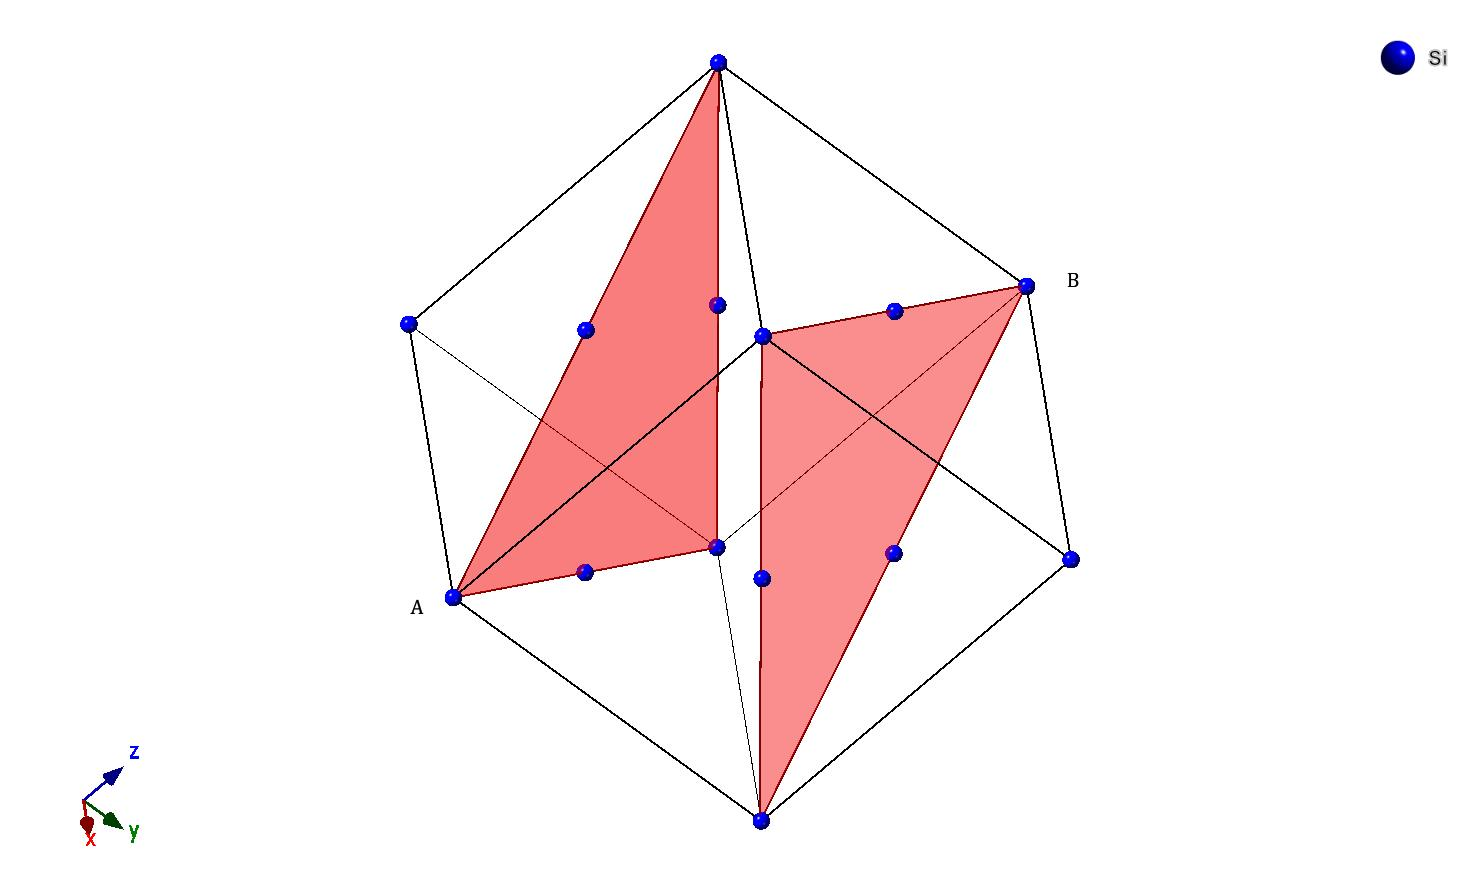
\includegraphics[width=0.5\textwidth]{fig/fcc_111.jpeg}
                    \caption{面心立方晶体单位晶胞以及$(111)面$。}
                    \label{面心立方晶体单位晶胞以及111面}
                \end{figure}
                
                \autoref{面心立方晶体单位晶胞以及111面}画出来面心立方晶体单胞内的两个相邻的$(111)$面,如果晶体上的原子
                简化成相切的小球,并且投影到$(111)$面上,则得到\autoref{面心立方111面堆垛}。三个相邻的$(111)$
                面的原子中心投影位置不同,为了区别,分别记作A、B、C,三个面也叫做A、B、C面。
                \begin{figure}[ht]
                    \centering
                    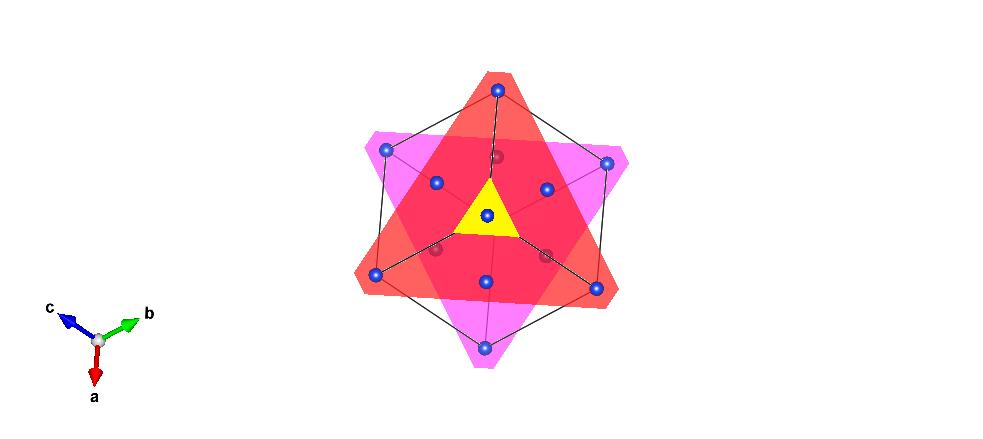
\includegraphics[width=0.7\textwidth]{fig/pile_up_of_planes_of_fcc_crystal.jpg}
                    \caption{面心立方的$(111)$堆垛情况。}
                    \label{面心立方111面堆垛}
                \end{figure}

                由\autoref{面心立方111面堆垛}可知,$(111)$面的堆垛规律为
                \begin{equation}
                    \cdots\cdots ABCABCABC\cdots\cdots 
                \end{equation}
                由于晶体的对称性,$(111)$面这种排列规律自然可以推广到所有的$\left\{ 111\right\}$
                晶面中去。

                晶面的正常堆垛次序被破坏时,就要出现堆垛层错或简称层错\index{层错}
                的晶格缺陷。面心立方晶体$\left\{ 111\right\}$面两种基本类型的层错
                可以表示为
                \begin{equation}
                    \cdots\cdots ABCACABC\cdots\cdots \label{面心立方层错形式1}
                \end{equation}
                和
                \begin{equation}
                    \cdots\cdots ABCACBCABC\cdots\cdots \label{面心立方层错形式2}
                \end{equation}
                \autoref{面心立方层错形式1}相当于从正常堆垛次序中抽掉一层晶面,因而称为
                抽出型层错\index{抽出型层错},层错中心位置位于缺少的晶面上;\autoref{面心立方层错形式2}
                相当于在正常堆垛次序中加入一层额外晶面,因而称为插入型层错\index{插入型层错},
                层错中心位置位于插入的晶面上。

                堆垛层破坏了晶体的完整性,是一种晶格缺陷,引起晶体能量的升高。与单位面积
                堆垛层错相联系的能量称为层错能\index{层错能}。从\autoref{面心立方层错形式1}
                和\autoref{面心立方层错形式2}可以看出,层错仅仅破坏了原子的次近邻关系,并
                没有破坏原子的最近邻关系,也即在层错处,只有从连续三层原子面的关系才能
                发现与正常堆垛次序的差别,如果仅仅取出相邻的两个原子面来看,无法观察到层错。
                因此层错虽然具有能量,但是与最近邻原子关系受到破坏的一般晶粒编辑的界面能相比,
                层错能要小得多。虽然目前理论计算层错能尚未解决,但是有一些估计层错能的实验方法。
                
                在薄晶体的电子显微镜衍衬法中,层错会引起特殊的干涉条纹,根据这种效应,
                可以之间看到层错能较小的晶体和合金中的层错。

                如果层错不贯穿整个晶体,而是中止余晶体内部,它就有一个边界线,如\autoref{Frank_partial_dislocation}
                所示。为了确定层错边界线的性质,围绕它作一个柏式回路。要注意回路的期待你应该选在层错面上,
                否则,回路在中途会穿过层错,造成困难。经过用柏式回路方法分析,可以证明上述层错都是具有 
                $\frac{1}{2}\langle 111 \rangle$小于面心立方晶体的初基矢量,所以这种类型的位错称为
                Frank偏位错\index{偏位错!Frank偏位错}。一般称与抽出型层错相联系的偏位错为负Frank偏位错,
                而与插入型层错相联系的偏位错被称为正Frank偏位错。Frank偏位错的柏式矢量与位错线垂直,因而总是
                刃型,但是它们不能滑移,因为如果滑移,就要离开所在的$(111)$面,并且在经过的路径上造成严重的
                原子错排,但是它们可以通过吸收或放出点缺陷在包含它们的$(111)$面作攀移运动。
                \begin{figure}[ht]
                    \centering
                    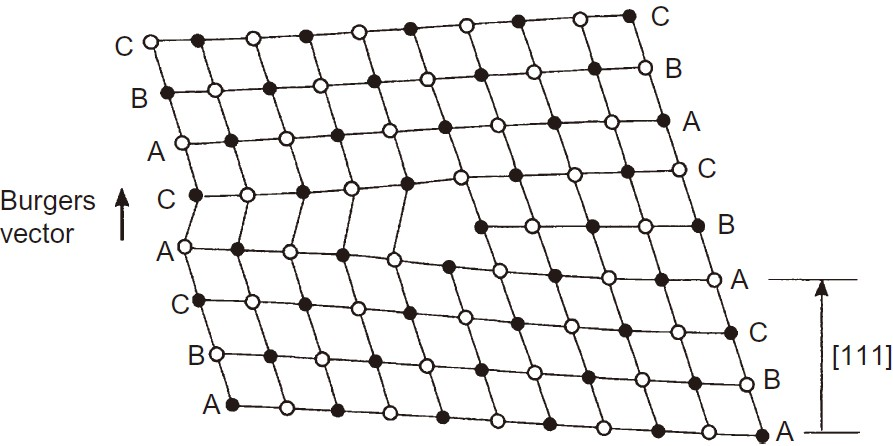
\includegraphics[width=0.5\textwidth]{fig/Formation_of_a_Frank_partial_dislocation.jpg}
                    \caption{密排面的部分原子缺失导致了$\frac{1}{3}\langle111\rangle$偏位错柏式矢量的形成。}
                    \label{Frank_partial_dislocation}
                \end{figure}
                
                面心立方晶体中另一种重要的偏位错为Shockley偏位错\index{Shockley偏位错},柏式矢量为 $\frac{1}{6}\langle 112 \rangle$。
                \autoref{Shockley偏位错模型}中晶体左上角相对其它部分移动了$\frac{1}{6}[\bar{2}11]$,结果
                在晶体左侧$(111)$晶面的堆垛次序发生改变,出现了一片与抽出型层错相同的层错。
                对这篇层错的边界线应用柏式回路方法进行分析,发现它具有的柏式矢量为$\frac{1}{6}[\bar{2}11]$,
                所以这片层错的边界线就是Shockley偏位错。
                \begin{figure}[ht]
                    \centering
                    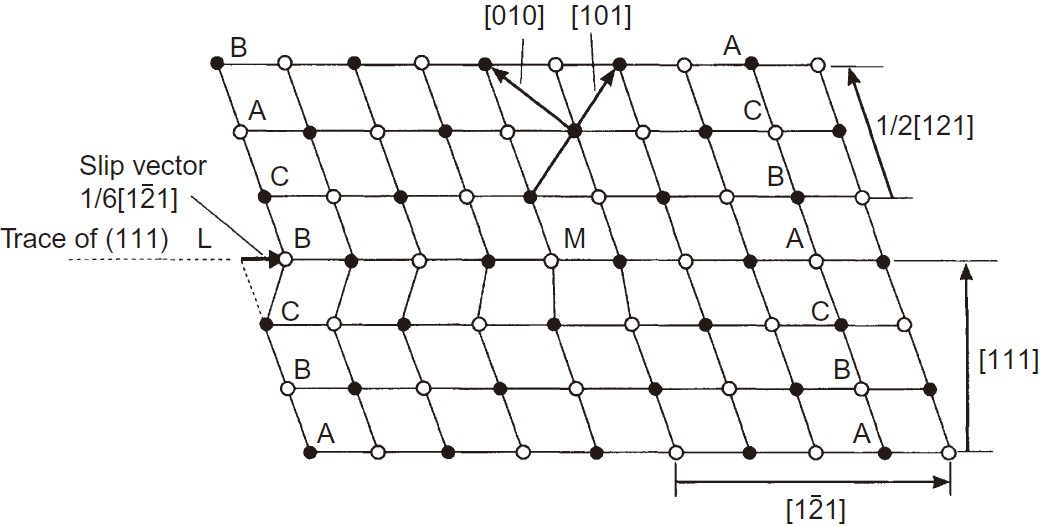
\includegraphics[width=0.5\textwidth]{fig/Formation_of_a_Shockley_partial_dislocation.jpg}
                    \caption{Shockley偏位错模型。}
                    \label{Shockley偏位错模型}
                \end{figure}
                
                \autoref{Shockley偏位错模型}中的位错为纯刃型位错,根据柏式矢量和位错线夹角的关系,也可以
                是螺型或是混合型位错,而且Shockley偏位错可以滑移,滑移面就是${111}$面,然而即使是刃型的
                Shockley偏位错也不能攀移,因为这也会造成严重的错排面。

                关于面心立方的位错总结如\autoref{面心立方的位错类型}
                \begin{table}[ht]
                    \begin{center}
                        \caption{面心立方的位错类型。}
                        \label{面心立方的位错类型}
                        \begin{tabular}{cccc}
                            \toprule
                            名称&全位错&Shockley偏位错&Frank偏位错 \\
                            \midrule
                            柏式矢量& $\frac{1}{2}\langle 110 \rangle$& $\frac{1}{6}\langle 211 \rangle$& $\frac{1}{3}\langle 111 \rangle$ \\
                            位错线&空间曲线&$\left\{ 111\right\}面上的曲线$&任意曲线\\
                            类型&3种&3种&仅有刃型\\
                            运动方式&滑移和攀移&滑移&攀移\\
                            形成方式&切变&$\left\{ 111\right\}$面上的滑移&插入或抽去一层\\
                            \bottomrule
                        \end{tabular}
                    \end{center}
                \end{table}

            \subsection{面心立方的扩展位错}
                面心立方全位错的柏式矢量为$\frac{1}{2}\langle 110\rangle$,可以通过
                位错翻译在$\left\{ 111\right\}$面上分解为两个Shockley偏位错,例如,在
                $(111)$面的$\frac{1}{2}[\bar{1}10]$可按
                \begin{equation}
                    \frac{1}{2}[\bar{1}10]\to\frac{1}{6}[\bar{2}11]+\frac{1}{6}[\bar{1}2\bar{1}]
                \end{equation}
                在分解之后,位错自身的能量减少$\frac{1}{6}$,这在能量上是可行的。而$(111)$面的4个柏式矢量都可以发生分解
                \begin{equation}
                    \begin{aligned}
                    \frac{1}{2}[110]\to\frac{1}{6}[211]+\frac{1}{6}[12\bar{1}]\\
                    \frac{1}{2}[\bar{1}01]\to\frac{1}{6}[\bar{2}11]+\frac{1}{6}[\bar{1}\bar{1}2]\\
                    \frac{1}{2}[0\bar{1}1]\to\frac{1}{6}[1\bar{2}1]+\frac{1}{6}[\bar{1}\bar{1}2]
                    \end{aligned}
                \end{equation}
                如\autoref{111面的全位错分解为Shockley偏位错}所示。
                \begin{figure}[ht]
                    \centering
                    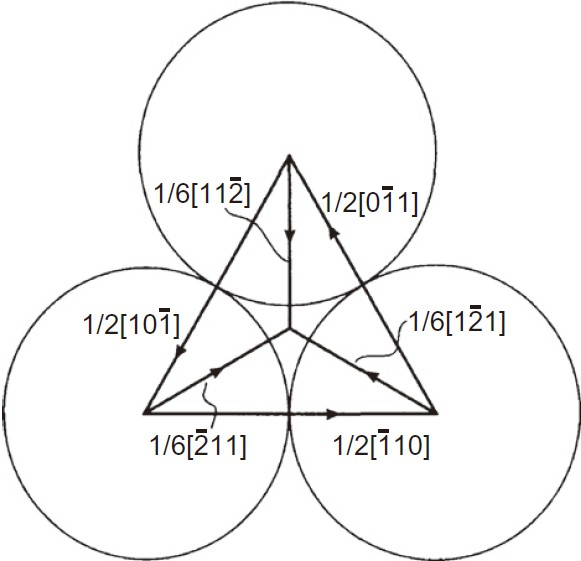
\includegraphics[width=0.5\textwidth]{fig/perfect_burgers_vector_to_shockley_partial_vector.jpg}
                    \caption{${111}$面的全位错分解为Shockley偏位错。}
                    \label{111面的全位错分解为Shockley偏位错}
                \end{figure}

                两个偏位错柏式矢量的夹角小于$\frac{\pi}{2}$可知,它们是互相排斥的;另一方面
                层错的表面张力却要求他们尽量靠近。随着两个片尾错的原理,相互排斥了逐渐降低,直到层错表面张力相等,位错
                之间的距离不再变化,这个平衡距离就是扩展位错的的扩展宽度。如果
                原位错与其柏式矢量的夹角为$\psi$,则两偏位错与柏式矢量的夹角分别为$\psi+\frac{\pi}{6}$
                和$\psi-\frac{\pi}{6}$,两个位错都化成刃型位错和螺型位错的分量,然后利用 \autoref{两个螺型位错之间的作用力}
                和\autoref{两个刃型位错之间的相互作用力},可以得到,片尾错之间的排斥力为
                \begin{equation}
                    F_{12}=\frac{\mu b^2(2-v)}{8\pi d(1-v)}\left[ 1-\frac{2v}{2-v}\cos{2\psi} \right],
                \end{equation}            
                其中$d$为两位错间距,$b$为偏位错强度。平衡时,$F_{12}$等于层错的表面
                张力,而表面张力与层错能$\gamma$像等,所以$F_{12}=\gamma$,代入上式,
                解出扩展宽度为
                \begin{equation}
                    d=\frac{\mu b^2(2-v)}{8\pi \gamma(1-v)}\left[ 1-\frac{2v}{2-v}\cos{2\psi} \right],
                \end{equation}
                由此可见,位错的扩展宽度与层错能成反比。

                扩展位错的运动很简单,实际上就是两个偏位错的运动。但是如果扩展位错是由
                螺型位错分解而来,它还可以进行交滑移。这时扩展位错交滑移分两步:束集(扩展位
                错合并成全位错),交滑移(螺位错变换滑移面的运动),如\autoref{扩展位错的交滑移过程}所示。
                \begin{figure}[ht]
                    \centering
                    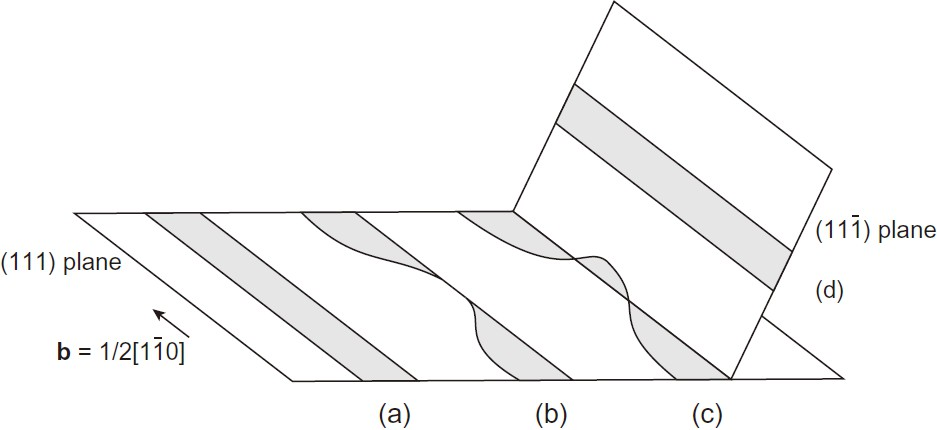
\includegraphics[width=0.7\textwidth]{fig/Four_stages_in_the_cross_slip_of_a_dissociated_dislocation.jpg}
                    \caption{螺位错从$(111)$面转移到$(11\bar{1})$面的四个过程。}
                    \label{扩展位错的交滑移过程}
                \end{figure}
                扩展位错交割时也先束集。所以层错能小,扩展位错宽度大,不易束集,不易运
                动,不易交割。
            \subsection{面角位错}
                
                假设在两个不同的$\left\{ 111\right\}$滑移面上有两个完整位错,如\autoref{压杆位错的形成}所示。
                如果两个位错在滑移过程中相交,形成一个新的位错$\frac{1}{2}[0\bar{1}1]$,由原来的两个柏式矢量相加得到。
                而且是一个刃型位错。这个面上的点阵阻力很大,无法滑移,这和位错也成为面角位错\index{面角位错}。
                \begin{figure}[ht]
                    \centering
                    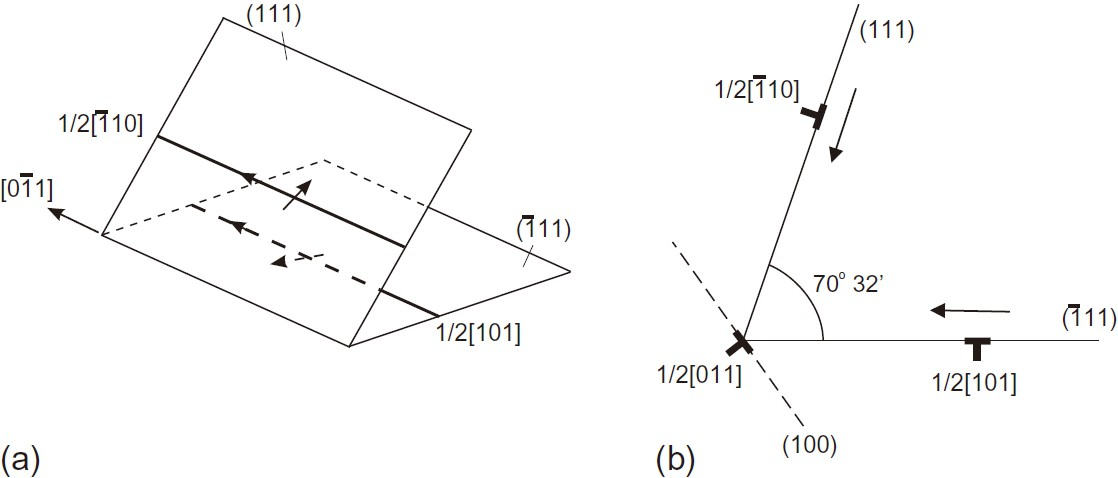
\includegraphics[width=0.7\textwidth]{fig/Formation_of_a_Lomer_sessile_dislocation.jpg}
                    \caption{压杆位错的形成。}
                    \label{压杆位错的形成}
                \end{figure}

                若为两个扩展位错相遇,则领头的两个位错合成新位错,滑移面由于阻力大而不能滑移。
                两个跟着的扩展位错也将受牵制而不动,组态不动,成为其它滑移的障碍物,面角位错也是加工硬化现象的一个重要原因。